% !TEX root = perelman-geometry.tex
%!TEX TS-program = pdflatex
%!TEX encoding = UTF-8 Unicode

\setchapterpreamble[o]{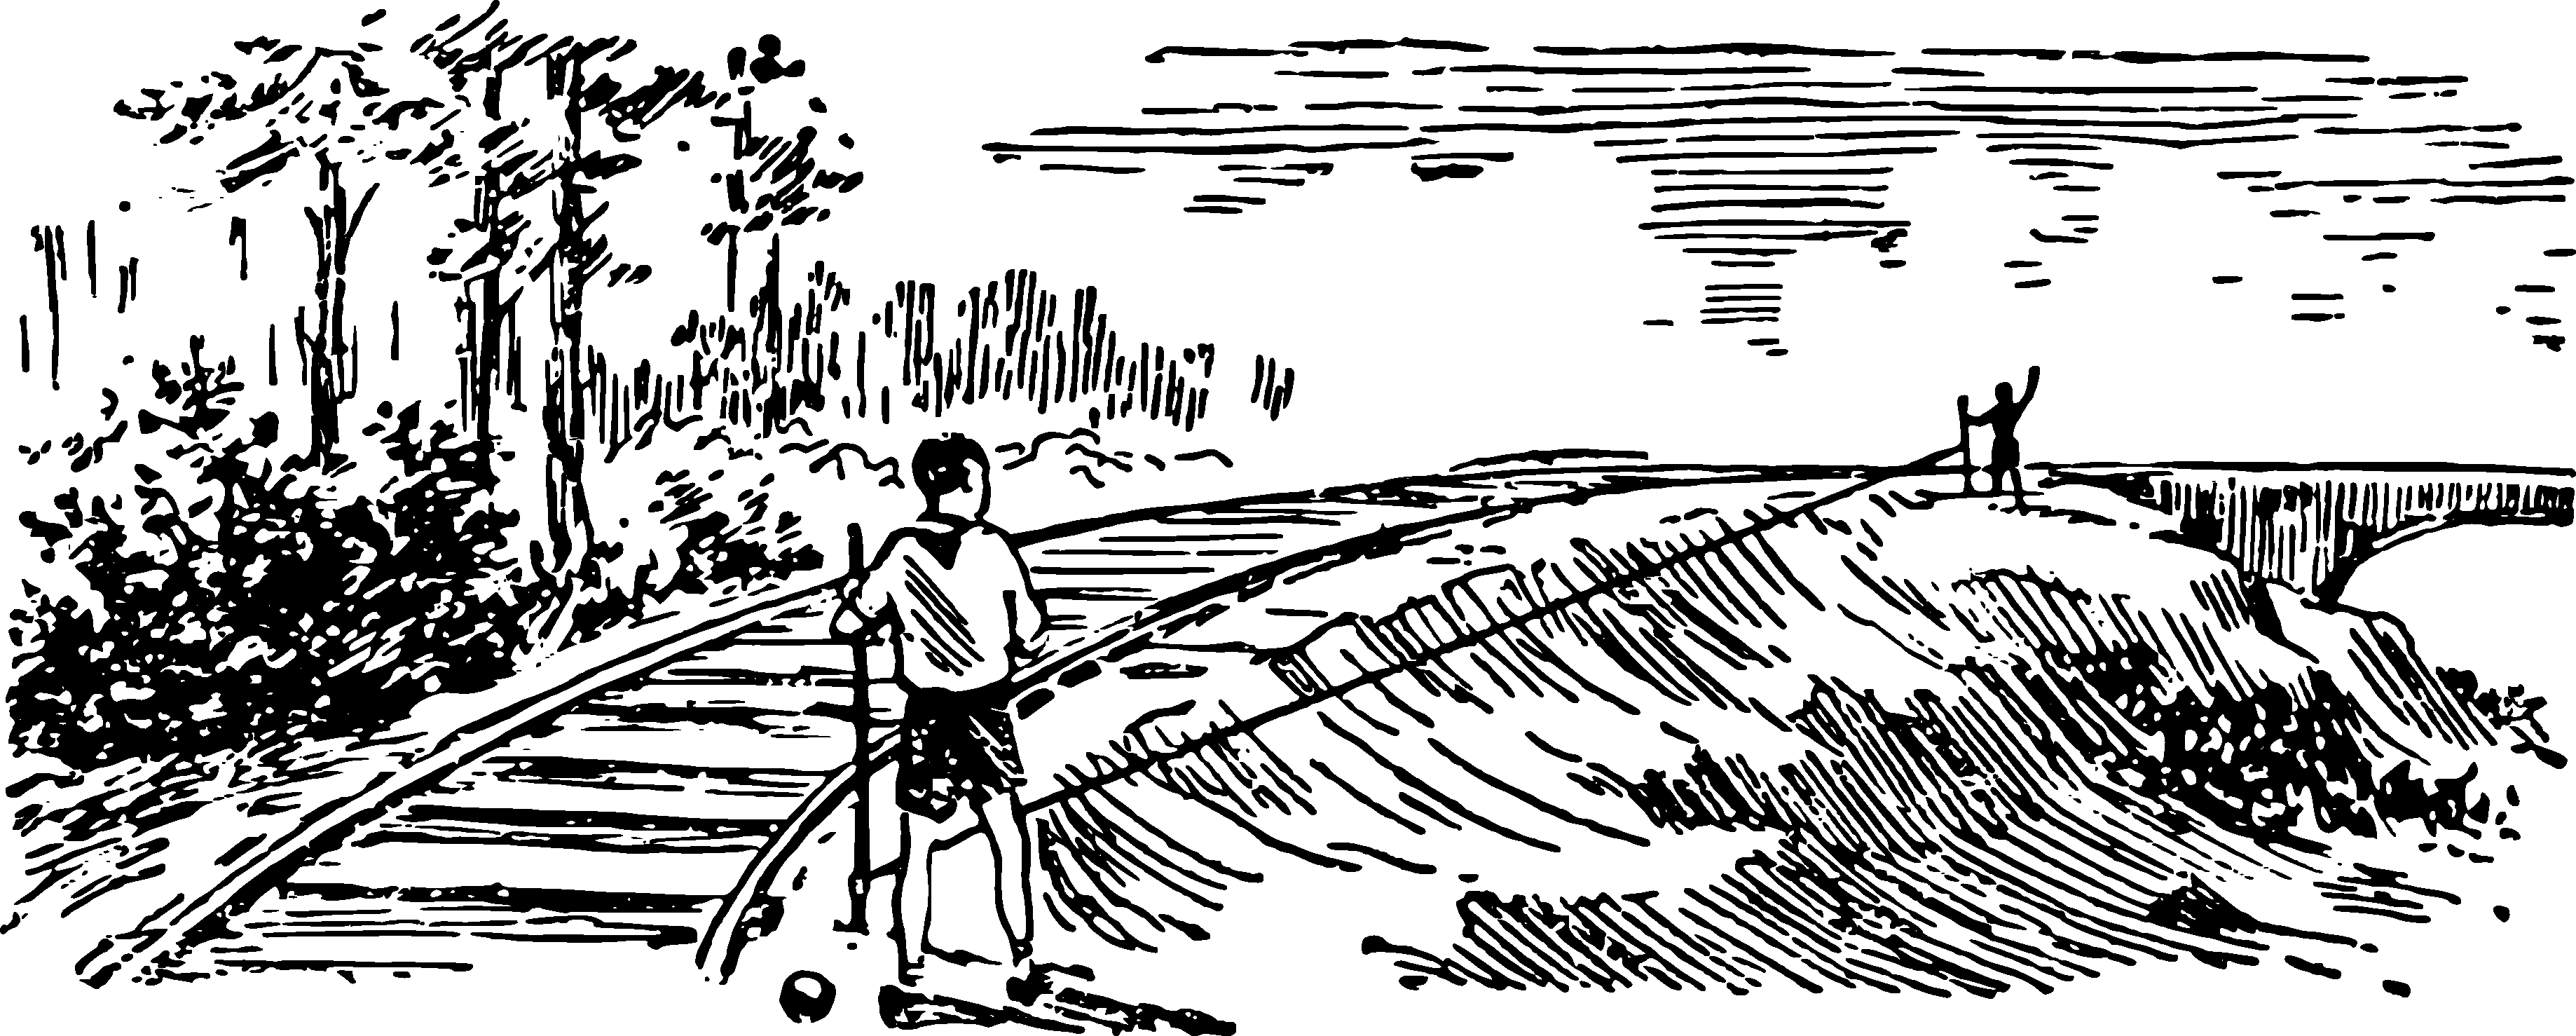
\includegraphics[width=1.2\textwidth]{figures/ch-04/fig-ch-04-head.pdf}\bigskip}

\chapter{Geometry on the Road}
\label{ch-04}

\section{The art of measuring by steps}
\label{sec-4.1}


While out for a countryside walk along a railway track or on a highway, you can perform a series of interesting geometric exercises.

First, use the highway to measure the length of your step and walking speed. This will allow you to -- measure distances by steps -- an art that is acquired quite easily after a short practise. The main thing here is to get used to making steps of the same length every time, i.e., to adopt a certain `measured' gait.

On the highway, every 100 meters, there is a white stone; by walking such a 100-meter interval with your usual `measured' step and counting the number of steps, you can easily find the average length of your step. Such measurement should be repeated annually, for example, every spring, because the length of a step, especially in young people, does not remain constant.

It is worth noting an interesting relationship discovered by repeated measurements: the average length of an adult's step is approximately half of their height, measured to eye level. For example, if a person's height to their eyes is 1 meter 40 centimetres, then the length of their step is about 70 centimetres. It's interesting to verify this rule whenever possible.

In addition to knowing the length of your stride, it's also useful to know your walking speed -- the number of kilometres you cover per hour. Sometimes the following rule is used for this: we walk as many kilometeres per hour as we take steps in three seconds; for example, if we take four steps in three seconds, then we walk 4 km per hour. However, this rule is only applicable when the length of the stride is known. It's not difficult to determine it: denoting the length of the stride in meters as $x$, and the number of steps in three seconds as $p$, we have the equation
\begin{equation*}%
\frac{3600}{3} \cdot nx = n \cdot 1000, 
\end{equation*}
from which $1200x = 1000$ and $x = 1000/1200 \si{\meter}$, i.e., about 80—85 cm. This is a relatively large stride; people of tall stature make such strides. If your stride differs from 80—85 cm, then you will need to measure your walking speed in a different way, by determining the time it takes you to cover the distance between two roadside posts using a clock.

\section{Eye-meter}
\label{sec-4.2}

It's pleasant and useful not only to measure distances without a measuring tape, but also to estimate them directly by eye without measurement. This skill is achieved only through practice. In my school years, when I participated in summer excursions out of town with a group of friends, such exercises were very common for us. They were carried out in the form of a special sport, invented by ourselves -- in the form of a competition for the accuracy of the eye-meter. When we went out on the road, we would visually mark some roadside tree or other distant object, and the competition would begin.

``How many steps to the tree?'' someone from the participants would ask.

The rest would give their estimated number of steps, and then together count the steps to determine whose estimate was closer to the truth -- that person would be the winner. Then it was their turn to mark an object for the eye-meter distance estimation.

Whoever determined the distance more accurately than the others would receive one point. After 10 times, the points were counted: the one with the most points was considered the winner of the competition.

I remember that at first our distance estimates were given with rough errors. But very soon, much faster than expected, we sharpened our skills in the art of estimating distances by eye, making very few mistakes. Only with a sharp change in surroundings, for example, when transitioning from an open field to sparse forest or to a bush-covered clearing, when returning to dusty, narrow city streets, or at night, with the deceptive illumination of the moon, would we catch each other making significant errors. However, we soon learned to adapt to all circumstances, mentally taking them into account during eye-meter estimates. Finally, our group reached such perfection in eye-meter distance estimation that we had to completely abandon this sport: everyone guessed equally well, and the competitions lost their interest. But we acquired a decent eye-meter, which served us well during our wanderings in the countryside.

It's curious that eye-metering seems to be independent of visual acuity. Among our group was a nearsighted boy who not only didn't lag behind the others in the accuracy of eye-meter distance estimation but sometimes even emerged as the winner of the competitions. Conversely, a boy with perfectly normal vision couldn't master the art of determining distances by eye at all. Later, I had to observe the same phenomenon when estimating the height of trees using the eye-meter method: practising this with students -- not for play anymore, but for the needs of future professions -- I noticed that nearsighted individuals mastered this skill just as well as others. This can be a consolation for the nearsighted: without having perfect vision, they are still capable of developing quite satisfactory eye-metering skills.

Practising eye-metering distance estimation can be done at any time of the year, in any setting. Walking along the city streets, you can set yourself eye-metering tasks, trying to guess how many steps to the nearest lamp-post or to various objects along the way. In bad weather, you can effectively fill the time with such activities while traversing empty streets.

The military pay a lot of attention to eye-metering distance estimation: a good eye-meter is necessary for a scout, a marksman, an artilleryman. It's interesting to learn about the signs they use in the practise of eye-metering estimations. Here are a few notes from the artillery textbook:

``On-eye distances are determined either by the skill of distinguishing visible objects at different distances from the observer to a certain degree of clarity, or by estimating distances using some familiar visual stretch of 100–200 steps, which seems smaller the further away it is from the observer.''

``When determining distances based on the clarity of visible objects, it should be noted that objects illuminated or brighter in colour appear closer in terrain or on water; objects positioned higher than others; groups compared to individual objects and generally larger objects.''

\begin{figure}[h!]
\centering
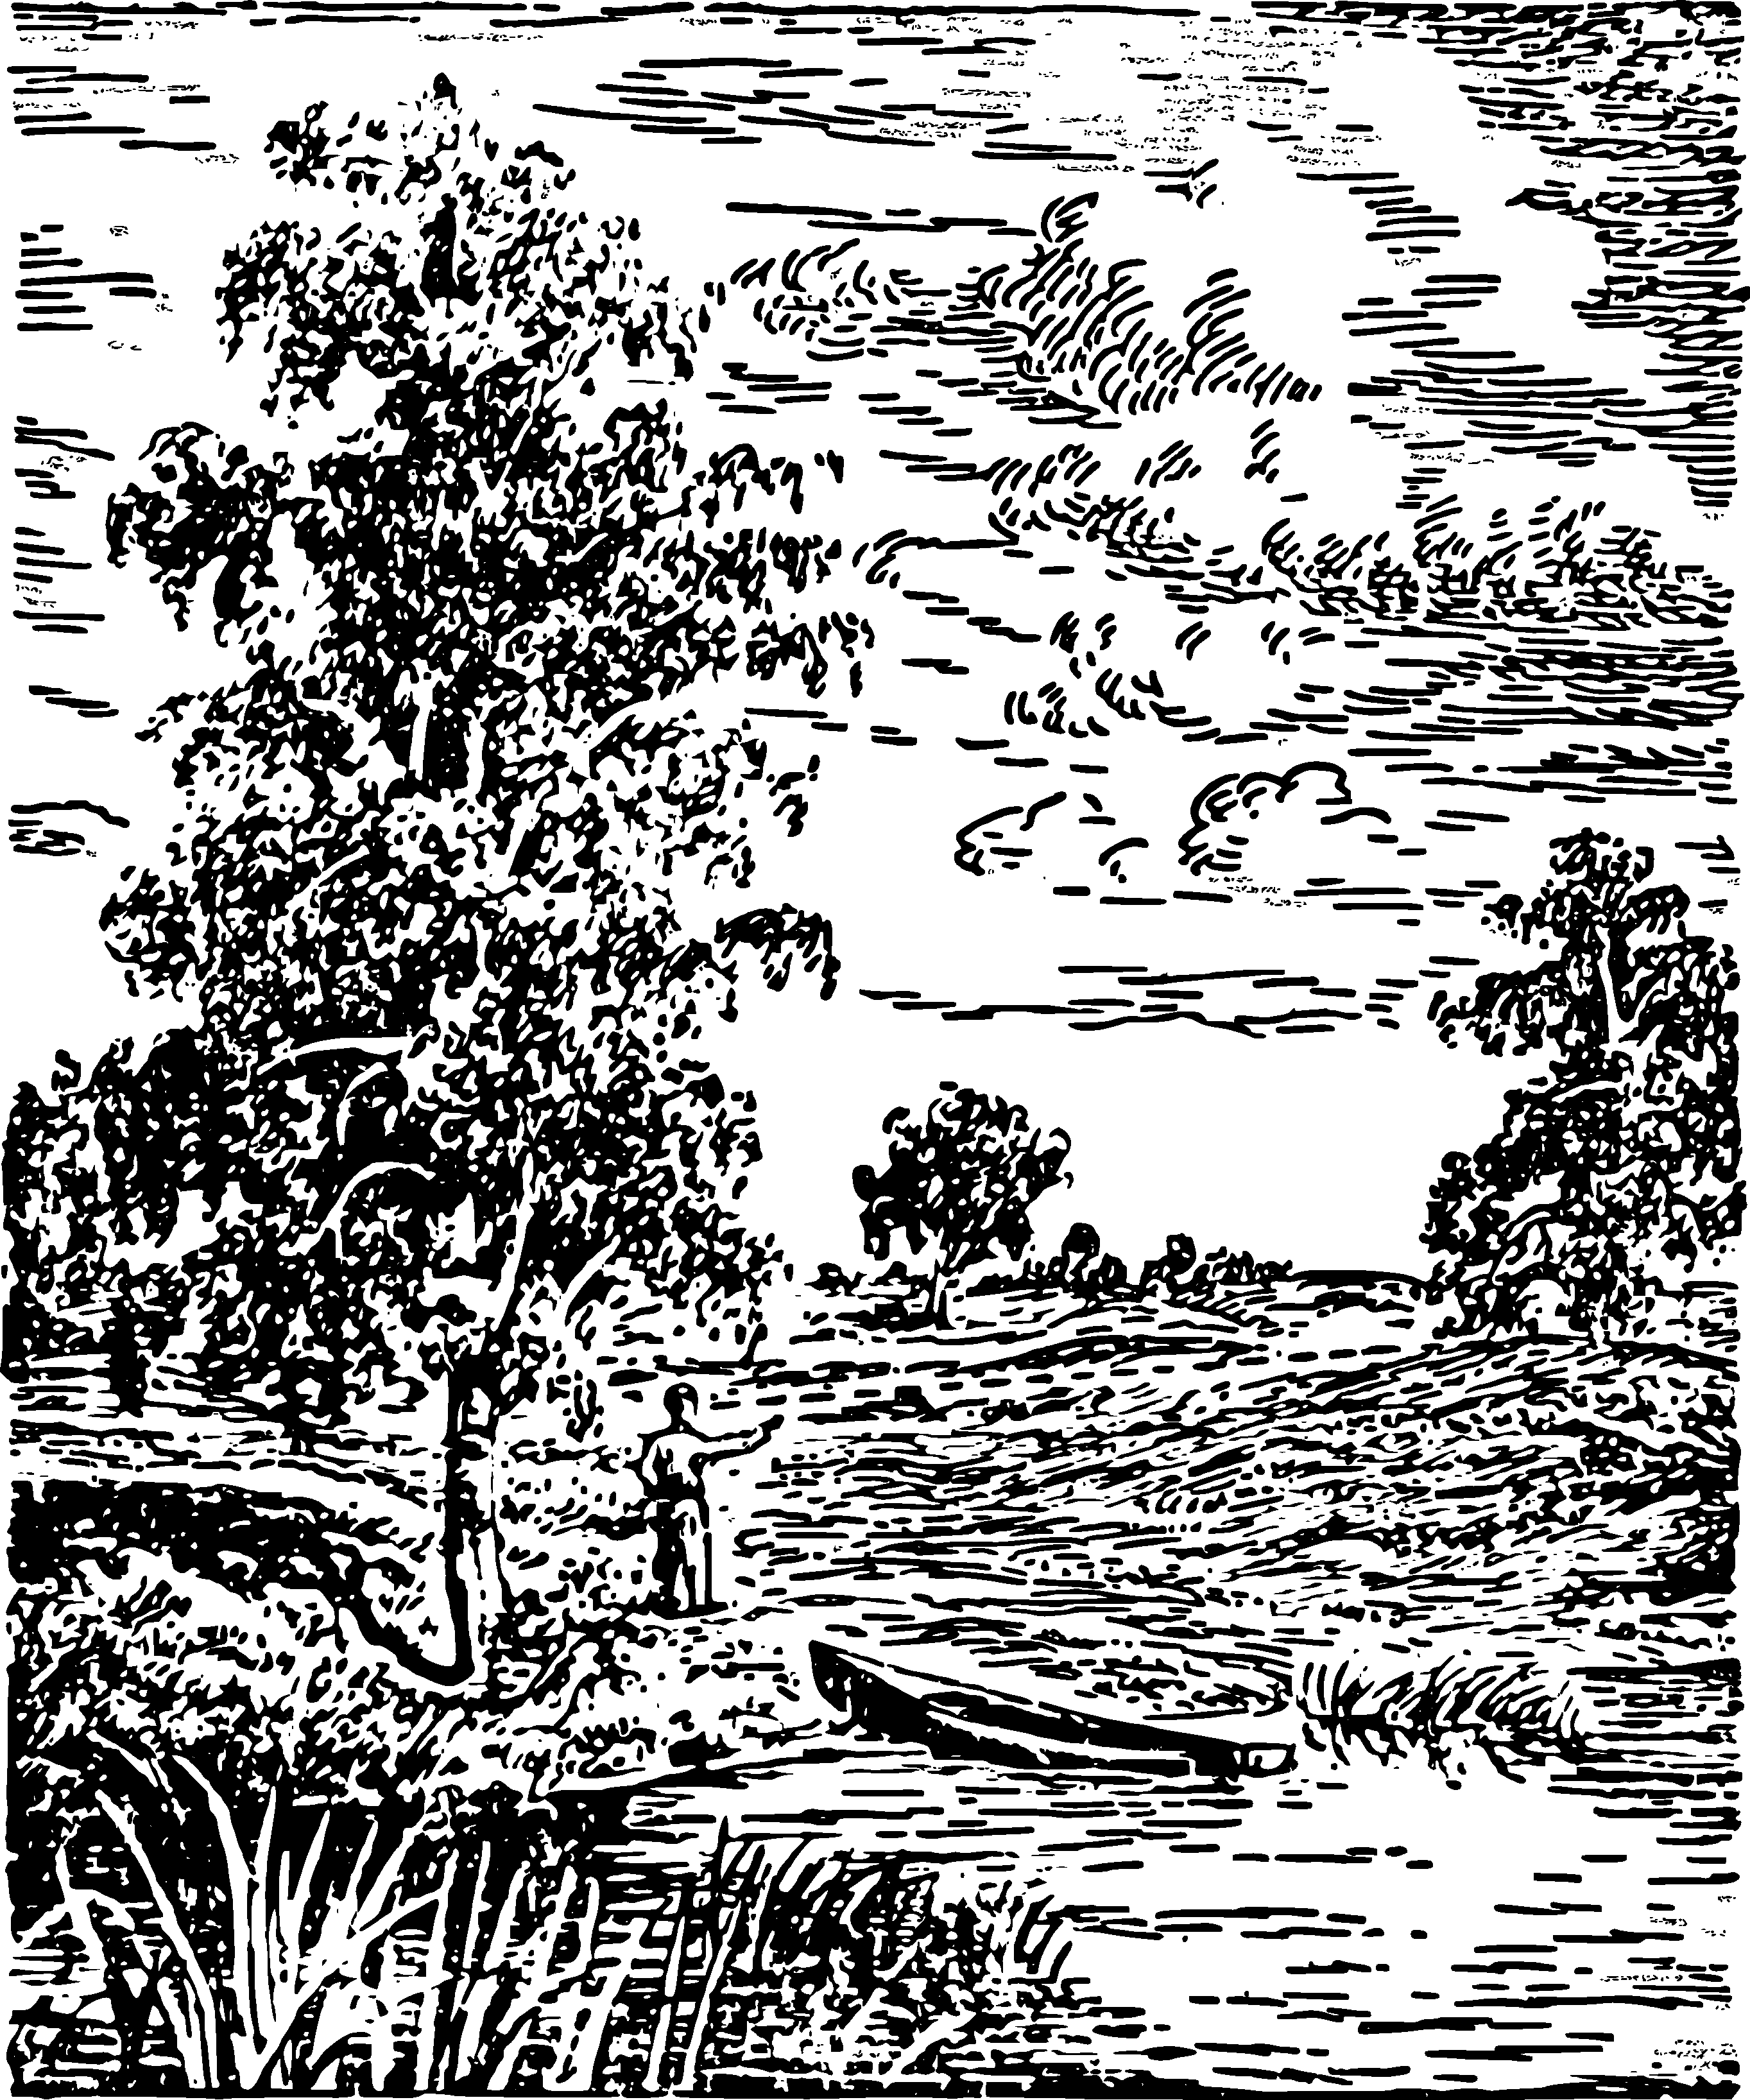
\includegraphics[width=0.9\textwidth]{figures/ch-04/fig-079.pdf}
\sidecaption{The tree behind the hillock seems close.\label{fig-079}}
\end{figure}

``You can follow the following signs: up to 50 steps, you can clearly distinguish people's eyes and mouth; at 100 steps, eyes appear as dots; at 200 steps, buttons and uniform details can still be distinguished; at 300 steps, the face is visible; at 400 steps, leg movements can be discerned; at 500 steps, the colour of the uniform is visible.''

At the same time, the most experienced eye may make an error of up to 10\% in either direction of the determined distance.


\begin{figure}[h!]
\centering
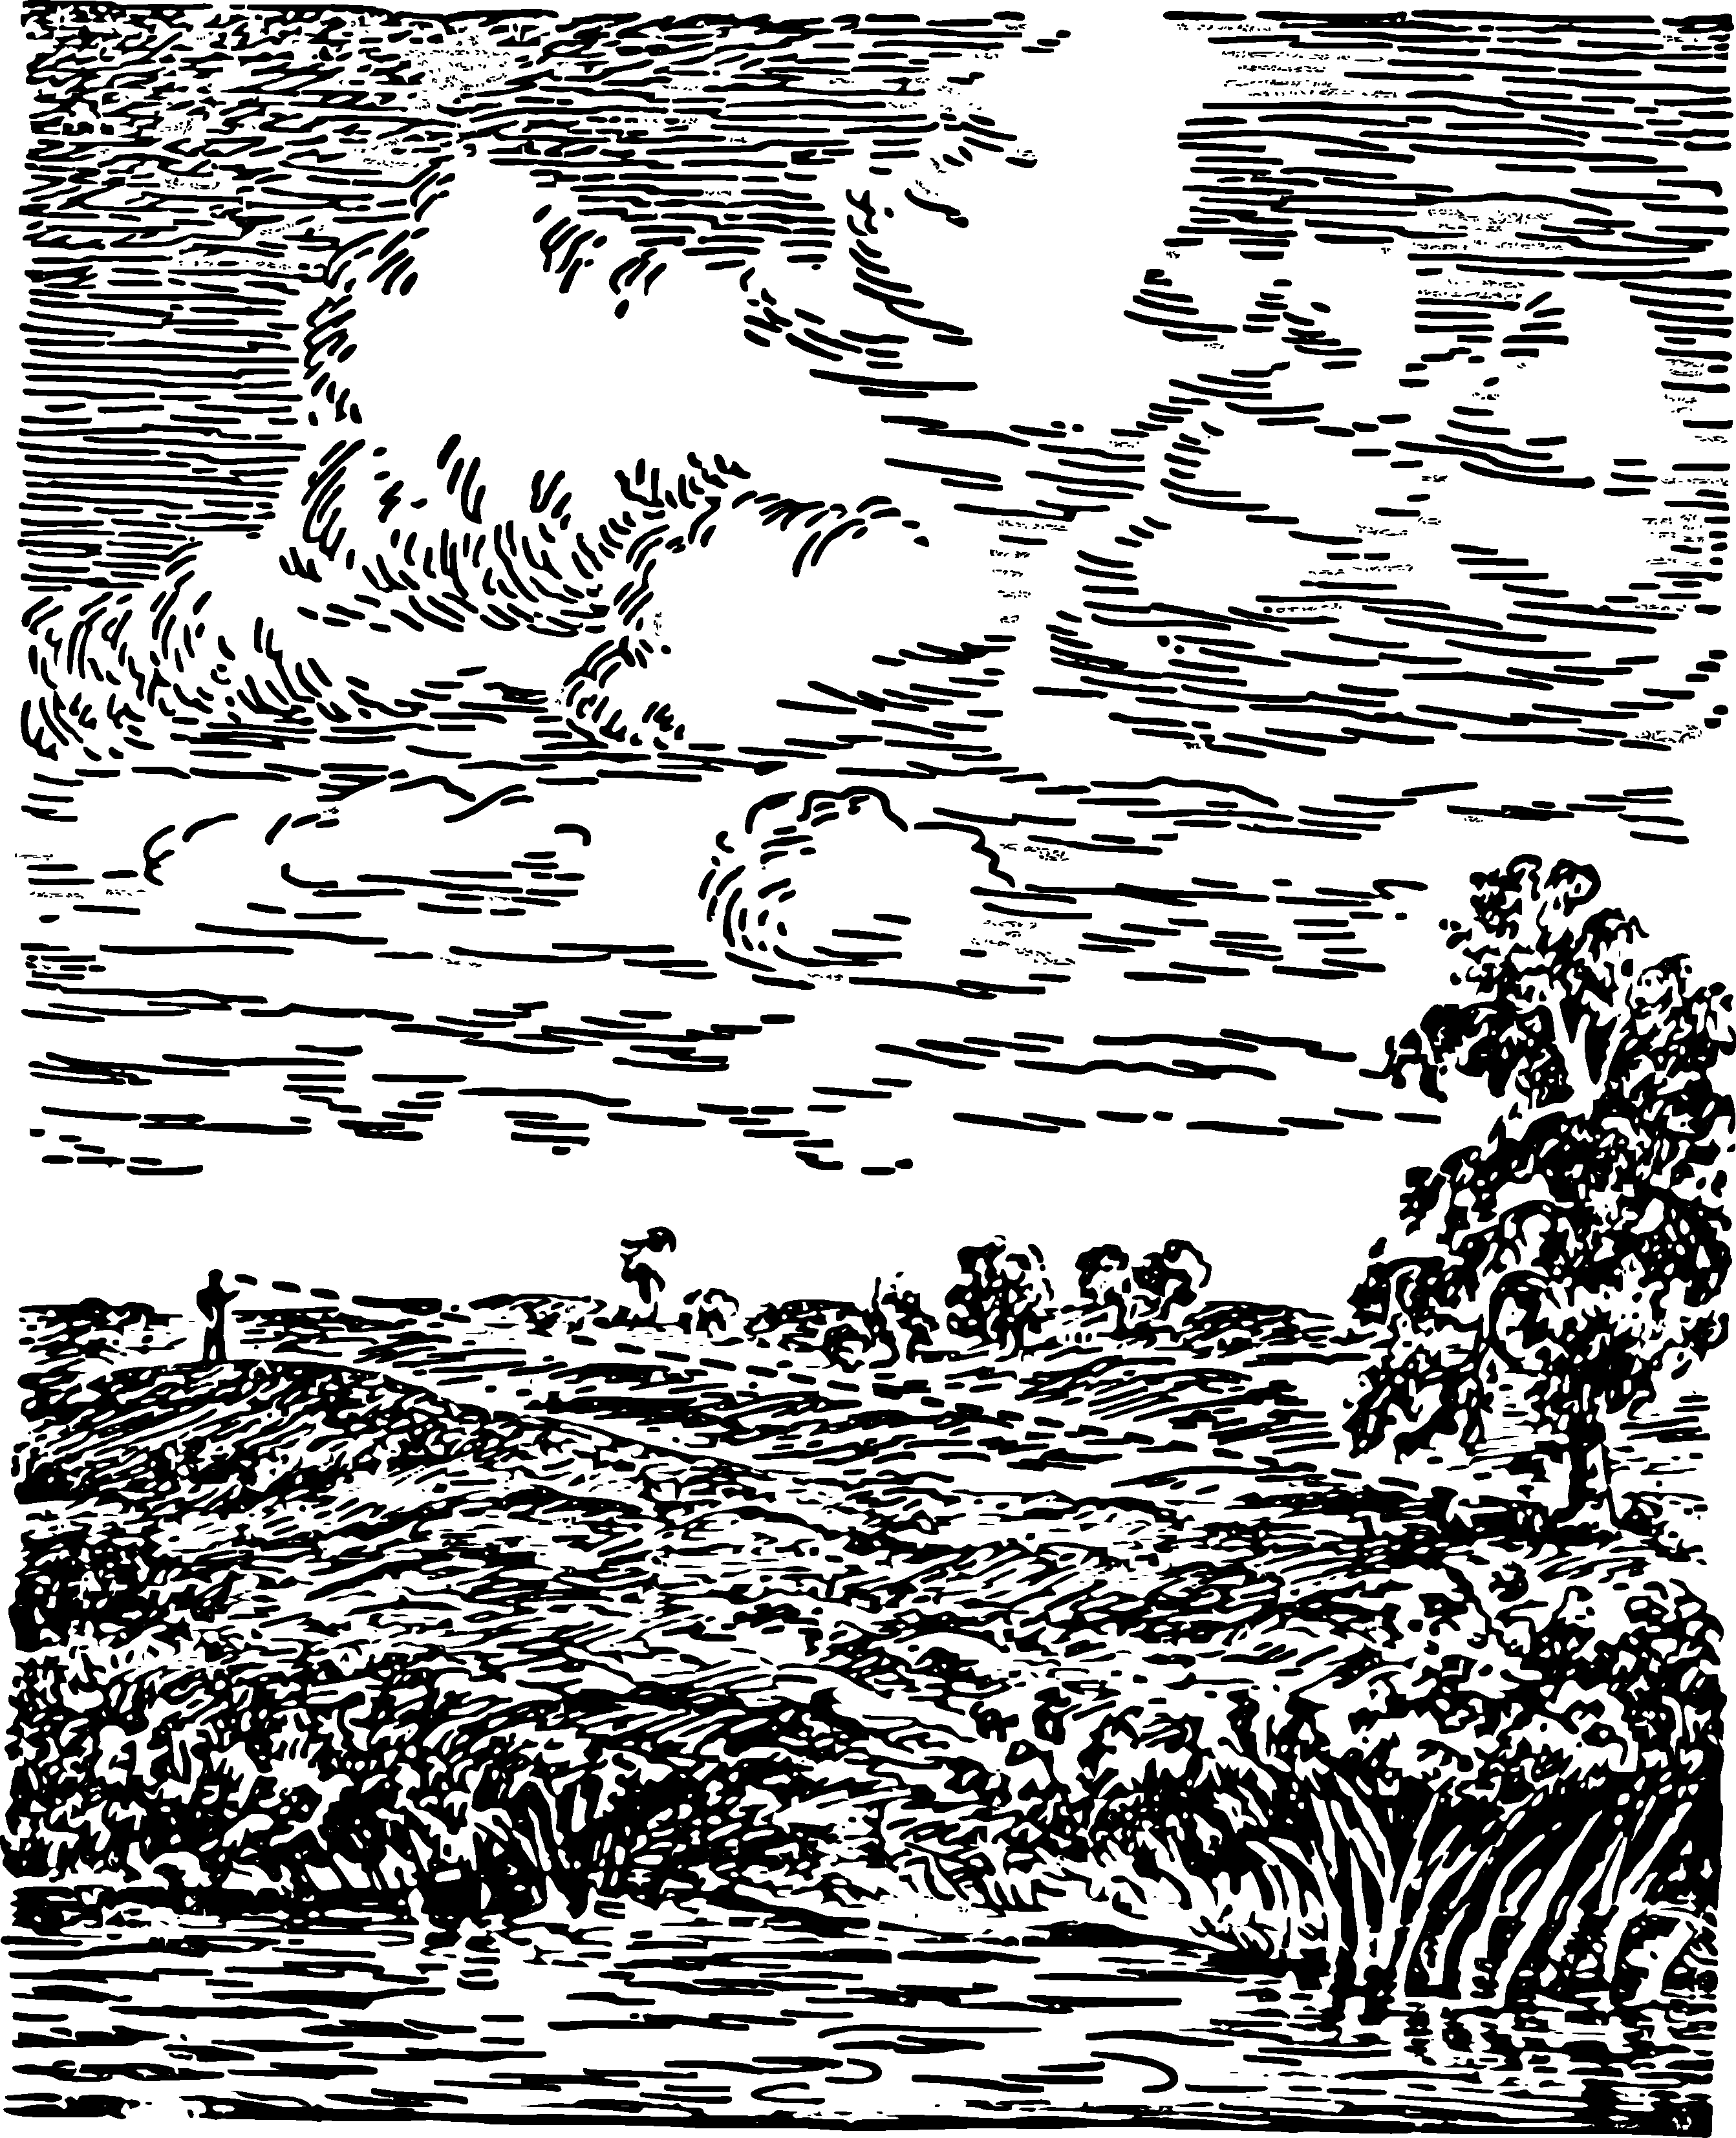
\includegraphics[width=0.9\textwidth]{figures/ch-04/fig-080.pdf}
\sidecaption{Climb up the hill, and the tree is still the same distance away.\label{fig-080}}
\end{figure}

There are cases, however, when eye-metering errors are much more significant. Firstly, when determining distance on a uniform, completely one-coloured surface -- on the smooth surface of a river or lake, on a clean sandy plain, on a densely overgrown field. Here, the distance always seems smaller than the true one; estimating it by eye, we make an error of two-fold, if not more. Secondly, errors are easily possible when determining the distance to an object whose base is obscured by a railway embankment, a small hill, a building, or any other elevation. In such cases, we involuntarily consider the object to be not behind the elevation, but on it itself, and therefore make an error again in the direction of reducing the determined distance (\figr{fig-079} and \figr{fig-080}).

In such cases, relying on the eye-meter is dangerous, and resorting to other methods of distance estimation, which we have already discussed and will continue to discuss, becomes necessary.


\section{Slopes}
\label{sec-4.3}

Alongside the railway track, besides the mile (more precisely -- kilometre) posts, you also see other low poles with inscriptions on small boards, like those shown in \figr{fig-081}.

\begin{figure}[h!]
\centering
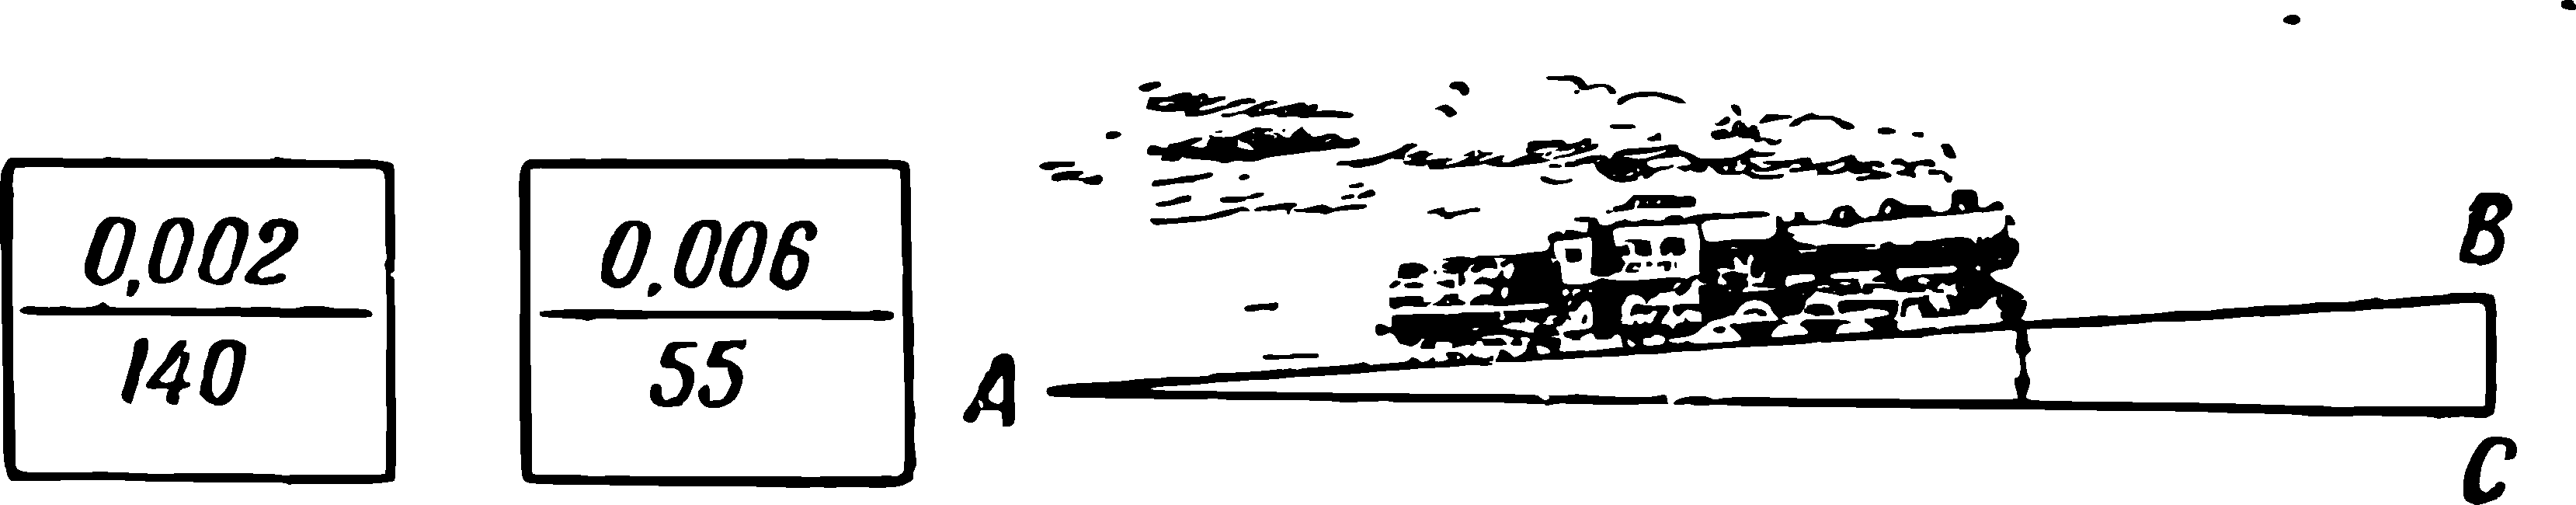
\includegraphics[width=0.9\textwidth]{figures/ch-04/fig-081.pdf}
\sidecaption{``Slope Signs.''\label{fig-081}}
\end{figure}


These are `slope signs.' In the first one, for example, the upper number 0.002 means that the gradient of the track here (in which direction -- indicated by the position of the board) is equal to 0.002: the track rises or descends by 2 mm for every thousand millimetres. And the lower number 140 indicates that such a gradient extends for 140 m, where another sign is placed with a notation of a new gradient. (When roads were not yet reorganised according to the metric system, such a board indicated that over a distance of 140 fathoms, the track rises or descends every fathom by 0.002 fathoms.) The second board with the inscription 0.006/55 indicates that over the next 55 m, the track rises or descends by 6 mm for every meter.

Knowing the meaning of the slope signs, you can easily calculate the difference in height between two adjacent points on the track marked by these signs. In the first case, for example, the height difference is $0.002 \times 140 = \SI{0.28}{\meter}$; in the second case -- $0.006 \times 55 = \SI{0.33}{\meter}$.

In railway practise, as you can see, the magnitude of the track gradient is not determined in degrees. However, it is easy to convert these track gradient markings into degrees. If $AB$ (\figr{fig-081}) is the path line, $BC$ is the height difference between points $A$ and $B$, then the inclination of the path line $AB$ to the horizontal line $AC$ will be marked on the post by the ratio $BC/AC$. Since angle $A$ is very small, we can take $AB$ and $AC$ as radii of a circle, the arc of which is $BC$.\sidenote{To another reader, it may seem perhaps unacceptable to consider the inclined $AB$ equal to the perpendicular $AC$; Therefore, it is instructive to ensure how small the difference in length between $AC$ and $AB$ is when $BC$ is, for example, $0.01$ of $AB$. By the Pythagorean theorem, we have:
\begin{align*}%
AC^{2} & = \sqrt{AB^{2} - \frac{AB^{2}}{100}}\\
& = \sqrt{0.9999\, AB^{2}} \approx 0.99995 \, AB^{2}.
\end{align*}
The difference in length is only $0.00005$. For approximate calculations, such a small error can certainly be neglected.
} Then the calculation of angle $A$, if the ratio $BC:AB$ is known, will not be difficult. With a slope, for example, marked as 0.002, we reason as follows: with an arc length equal to 1/57 radius, the angle is \ang{1} (see page~\pageref{fig-062}); what angle corresponds to an arc of 0.002 radii? We find its value $x$ from the proportion 
\begin{align*}%
\frac{x}{\ang{1}} & = \frac{0.002}{1/57},\,\, \text{from where}\\
x & = 0.002 \times 57 = \ang{0.11},
\end{align*}
i.e., about \ang{;7}.
 
Only very small gradients are allowed on railway tracks. We have set the maximum gradient at 0.008, i.e., in degrees, $0.008 \times 57$ -- less than \ang{0.5}: this is the maximum gradient. Only for the Transcaucasian Railway, gradients up to 0.025 are allowed as an exception, which corresponds to almost \ang{1.5} in degrees.

Such insignificant gradients are completely unnoticed by us. A pedestrian begins to feel the slope under their feet only when it exceeds 57/24: this corresponds to approximately \ang{2.5} in degrees.

Having walked along the railway track for several kilometres and noted the observed gradient signs, you can calculate how much you have ascended or descended in total, i.e., what is the difference in height between the starting and ending points.


\ques You started a walk along the railway track at a post marked with an ascent of 0.004/153 miles and encountered the following signs further along\sidenote{Sign 0.000 means a horizontal section of the path (``platform'').}: 
\begin{small}
\begin{center}
\begin{tabular}{ccccc}
\toprule
Platform & Ascent & Ascent & Platform & Descent\\
\midrule 
$\dfrac{0.000}{60}$ & $\dfrac{0.0017}{84}$ & $\dfrac{0.0032}{121}$ & $\dfrac{0.000}{45}$ & $\dfrac{0.004}{210}$ \\
\bottomrule
\end{tabular}
\end{center}
\end{small}
You finished the walk at another slope sign. What distance did you travel, and what is the difference in height between the first and last signs?

\ans Total distance travelled: 
\begin{equation*}%
153 + 60 + 84 + 121+ 45 + 210 = \SI{673}{\meter}
\end{equation*}
You went up by
\begin{equation*}%
0.004 \times 153 + 0.0017 \times 84 + 0.0032 \times 121 = \SI{1.15}{\meter}
\end{equation*}
and descended:
\begin{equation*}%
0.004 \times 210 = \SI{0.84}{\meter}.
\end{equation*}
Therefore, in total, you ended up higher than the starting point by $1.15 - 0.84 = \SI{0.31}{\meter}$.

\section{Heap of Gravel}
\label{sec-4.4}

Heap of gravel at the edges of the road also presents an object worthy of attention for the ``geometer in the open air.'' By asking what volume the heap in front of you contains, you set yourself a geometric problem, quite intricate for someone accustomed to overcoming mathematical difficulties only on paper or on the blackboard. 

\begin{figure}[h!]
\centering
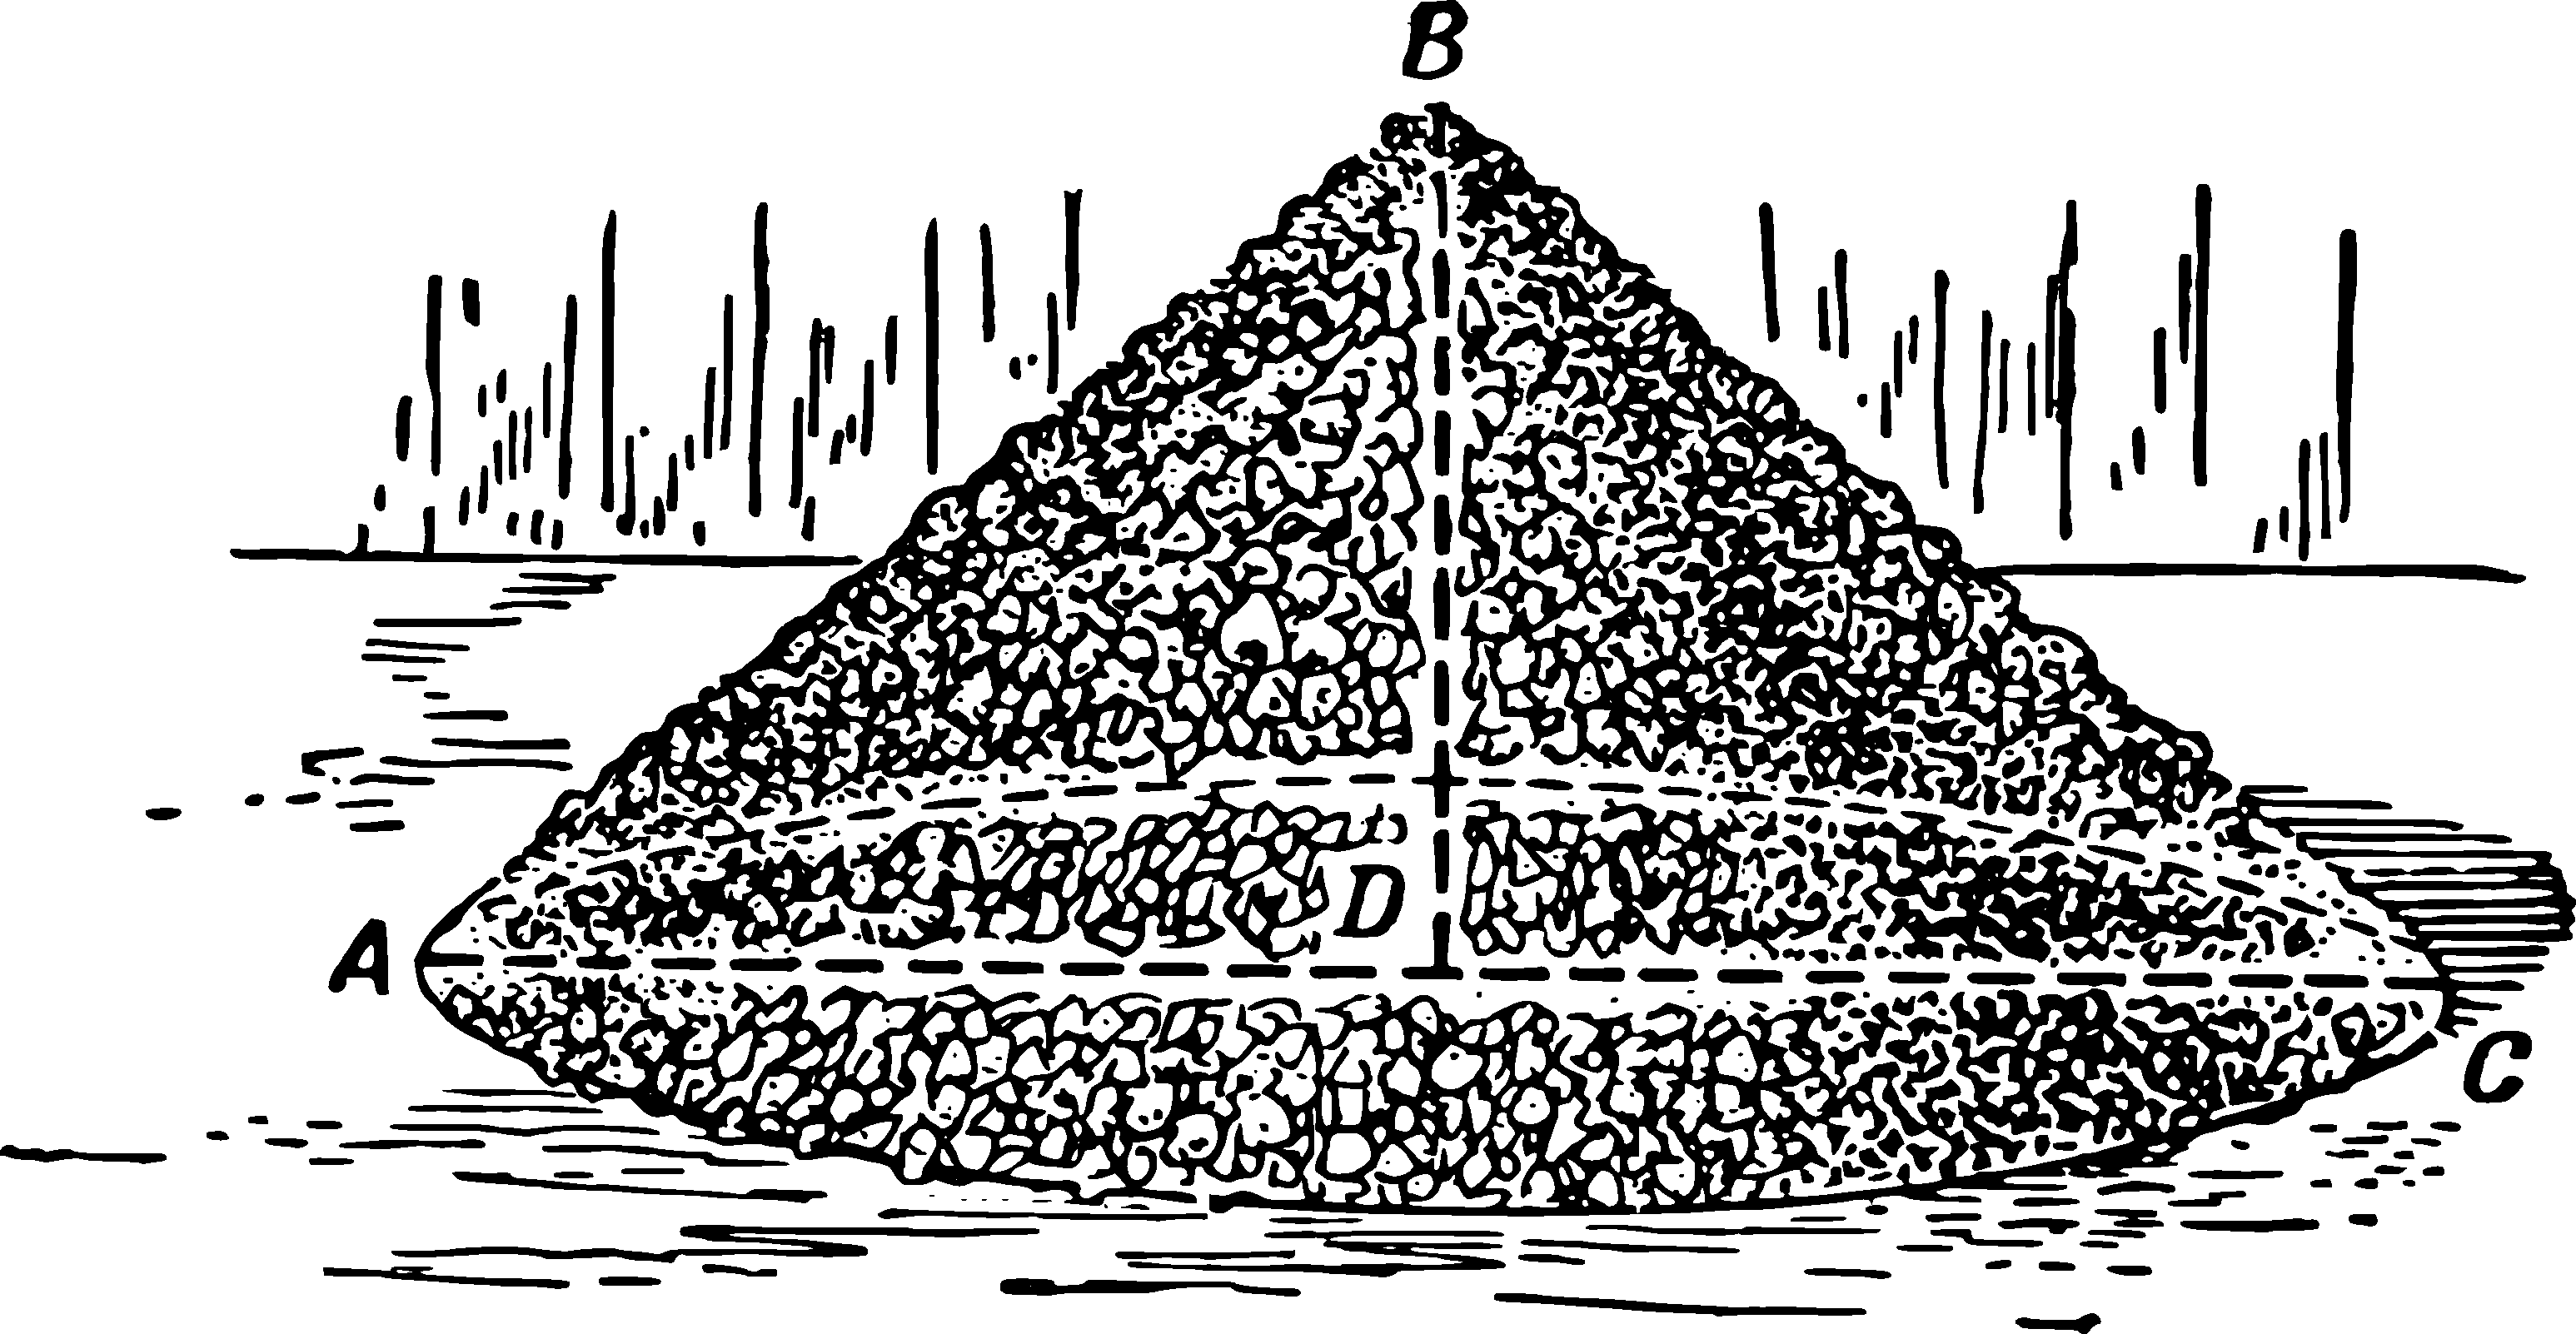
\includegraphics[width=0.9\textwidth]{figures/ch-04/fig-082.pdf}
\sidecaption{For the problem of the gravel heap.\label{fig-082}}
\end{figure}

You have to calculate the volume of a cone, the height and radius of which are not directly measurable. However, nothing prevents you from determining their value indirectly. You will find the radius by measuring the circumference of the base with a ruler or string and dividing it by $2\pi$.\sidenote{In practice, this action is replaced by multiplication by the reciprocal, if looking for the diameter, and by 0.159 if calculating the radius.} 

The height poses a greater challenge (\figr{fig-082}): you have to measure the length of the generatrix $AB$ or, as the road surveyors do, both generatrices $ABC$ at once (by laying the measuring tape over the apex of the heap), and then, knowing the radius of the base, calculate the height $BD$ using the Pythagorean theorem. Let's consider an example.

\ques The circumference of the base of a conical heap of gravel is 12.1 m; the length of the two generatrices is 4.6 m. What is the volume of the heap?

\ans The radius of the base of the heap is 
\begin{equation*}%
12.1 \times 0.159 \,\, \text{(instead of 12.1/6.28)} = \SI{1.9}{\meter}.
\end{equation*}
The height is 
\begin{equation*}%
\sqrt(2.3^{2} - 1.9^{2}) =  \SI{1.2}{\meter},
\end{equation*}
hence the volume of the heap is 
\begin{equation*}%
\frac{1}{3} \times 3.14 \times 1.9^{2} \times 1.2 =  \SI{4.6}{\meter\cubed}
\end{equation*}
(approximately 1/2 cubic fathoms in previous measurements).

Typically, the standard volume measurements for gravel heaps on our roads were 1/2, 1/4, and 1/8 cubic fathoms, i.e., in metric units, 4.8, 2.4, and 1.2 cubic meters.


\section{The Proud Hill}
\label{sec-4.5}

Looking at conical heaps of gravel or sand brings to mind an ancient legend of Eastern peoples, retold by Pushkin in \emph{The Miserly Knight}:

\begin{quote}
\emph{I read somewhere,\\
That once a king ordered his warriors\\
To carry earth by handfuls into a heap, --\\
And a proud hill rose up,\\
And the king could from the heights with joy survey\\
Both the valley, covered with white tents,\\
And the sea, where ships sailed.}
\end{quote}

This is one of those few legends in which, despite its seeming plausibility, there is not a grain of truth. It can be proven by geometric calculation that if some ancient despot had decided to undertake such an endeavour, he would have been discouraged by the meagerness of the result: before him would have risen such a pitiful pile of earth that no imagination could inflate it into the legendary ``proud hill''.

Let's make an approximate calculation. (How many warriors could an ancient king have? Ancient armies were not as numerous as they are today. An army of 100,000 people was already very impressive in size. Let's stick with this number, i.e., assume that the hill was composed of 100,000 handfuls. Grab the largest handful of earth and fill a glass with it: you won't fill it with just one handful. Let's assume that the handful of an ancient warrior equalled in volume 1/5 (\si{\deca\meter\cubed}). Hence, the volume of the hill is:
\begin{equation*}%
\frac{1}{5} \times 100000 = 20,000 \si{\deca\meter\cubed} = 20 \si{\meter\cubed}.
\end{equation*}
Thus, the hill represented a cone with a volume of no more than 20 cubic meters. Such a modest volume is already disappointing. But let's continue the calculations to determine the height of the hill. To do this, we need to know the angle formed by the generatrices of the cone with its base. In our case, we can assume it to be equal to the angle of natural slope, i.e., \ang{45}: steeper slopes cannot be allowed as the earth would collapse (it would be more plausible to take an even shallower slope, for example, one and a half). Stopping at an angle of \ang{45}, we conclude that the height of such a cone is equal to the radius of its base; therefore,
\begin{align*}%
20 & = \frac{\pi x^{3}}{3}, \,\, \text{Hence,}\\
x & = \sqrt[3]{\frac{60}{\pi}} =  2.4 \si{\meter}.
\end{align*}
One must possess a rich imagination to call a pile of earth 2.4 meters (1.5 human height) a ``proud hill.'' By making the calculation for the case of a one and a half slope, we would have obtained an even more modest result.

Attila had the most numerous army known in the ancient world. Historians estimate it to be 700,000 people. If all these warriors participated in building the hill, a heap taller than the one we calculated would have been formed, but not significantly: since the volume would be seven times larger than ours, the height would exceed the height of our heap by only 1.7 times; it would be equal to $2.4 \times 1.9 = 4.6$ meters. It is doubtful that a mound of such dimensions could satisfy the ambition of Attila.

From such small elevations, it was easy, of course, to see ``the valley covered with white tents''," but surveying the sea was possible only if the affair took place not far from the shore.

We will discuss how far one can see from a certain height in the sixth chapter.


\section{At a Road Curve}
\label{sec-4.6}

Neither highways nor railways ever make sharp turns; they always transition smoothly from one direction to another, without breaks, in an arc. This arc is usually part of a circle arranged so that the straight sections of the road serve as tangents to it. 

\begin{figure}[h!]
\centering
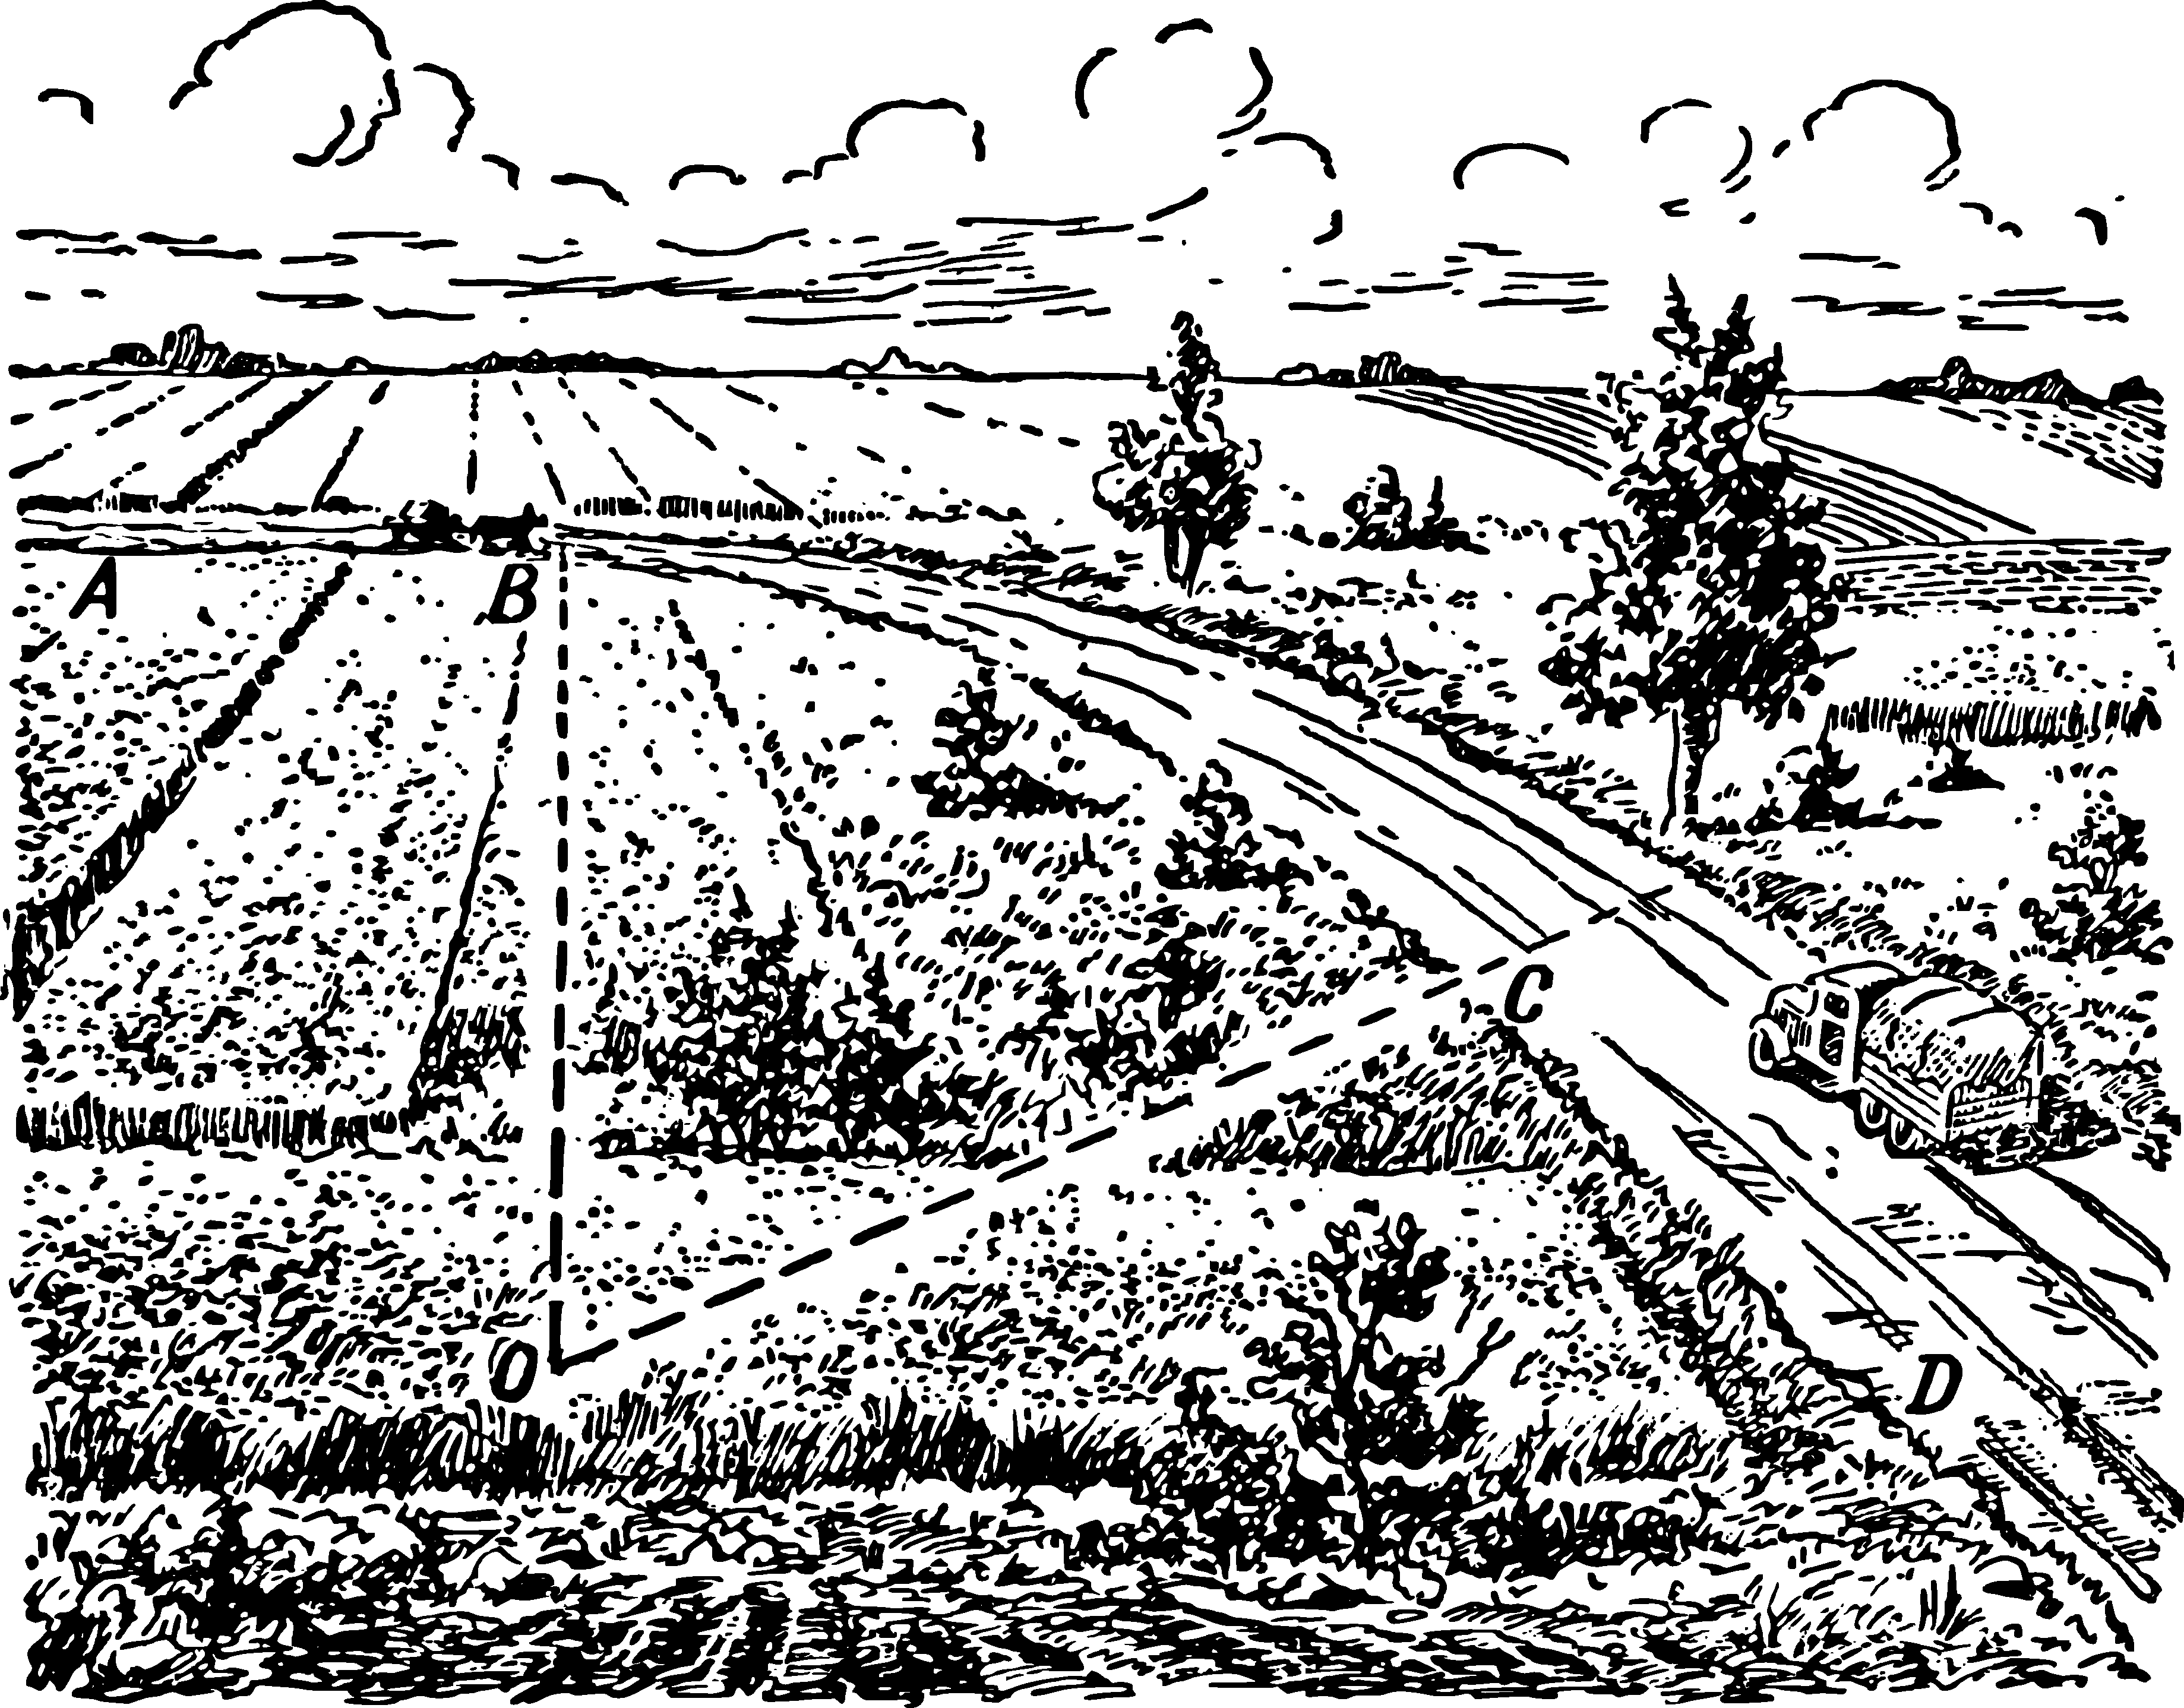
\includegraphics[width=0.9\textwidth]{figures/ch-04/fig-083.pdf}
\sidecaption{Road rounding.\label{fig-083}}
\end{figure}

For example, in \figr{fig-83}, the straight sections $AB$ and $CD$ of the road are connected by the arc $BC$ so that $AB$ and $CD$ touch (geometrically) this arc at points $B$ and $C$, i.e., $AB$ forms a right angle with radius $OB$, and $CD$ forms the same angle with radius $OC$. This is done, of course, to smoothly transition the path from a straight direction to a curved part and back again.

The radius of a road curve is usually taken to be quite large -- on railways, not less than 600 meters; the most common radius of curvature on the main railway track is 1000 or even 2000 m.



\section{Radius of Curvature}
\label{sec-4.7}


Standing near one of such curves, could you determine the magnitude of its radius? This is not as easy as finding the radius of an arc drawn on paper. On a drawing, it's simple: you draw two arbitrary chords and draw perpendiculars from their midpoints: the point of their intersection is known to be the centre of the arc; the distance from it to any point on the curve is the desired length of the radius.

But to make a similar construction on the ground would, of course, be very inconvenient: after all, the centre of the curve is 1-2 meters from the road, often in an inaccessible place. It would be possible to make the construction on a plan, but taking the curves off onto a plan is also not an easy task.

\begin{marginfigure}[-4cm]%[h!]
\centering
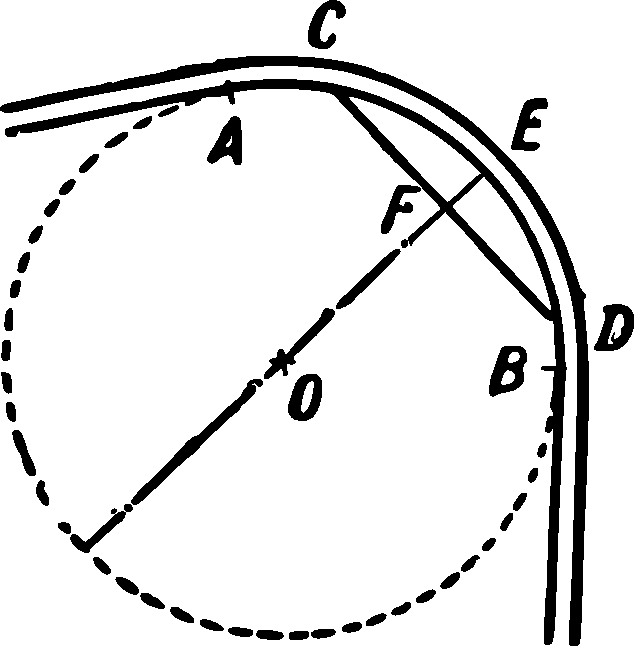
\includegraphics[width=\textwidth]{figures/ch-04/fig-084.pdf}
\sidecaption{To calculate the radius of curvature.\label{fig-084}}
\end{marginfigure}

All these difficulties are eliminated if one resorts not to constructing, but to calculating the radius. For this purpose, the following method can be used. We mentally supplement the arc $AB$ of the curve (\figr{fig-084}) to a circle. Connecting arbitrary points $C$ and $D$ of the arc of the curve, we measure the chord $CD$, as well as the ``arrow'' $EF$ (i.e., the height of the segment CED). From these two data, it is already not difficult to calculate the desired length of the radius.

Considering the lines $CD$ and the diameter of the circle as intersecting chords, we denote the length of the chord by $a$, the length of the arrow by $h$, the radius by $R$; we have:
\begin{align*}%
\frac{a^{2}}{4} & = h(2R - h),\,\,\text{from where}\\
\frac{a^{2}}{4} & = 2Rh - h^{2},\text{and the desired radius}\sidenote{This could have been obtained in another way — from a right triangles $COF$, where $OS=R$, $CF= a/2$, $OF = R - h$.
 According to the Pythagorean theorem 
\begin{align*}%
R^{2} & = (R -h)^{2} + \left(\frac{a}{2}\right)^{2}, \,\, \text{from where}\\
R^{2} & = R^{2} - 2Rh + h^{2} + \frac{a^{2}}{4},\\
R & = \frac{a^{2} + 4h^{2}}{8h}
\end{align*}}\\
R & = \frac{a^{2} + 4h^{2}}{8h}.
\end{align*}
For example, with an arrow of 0.5 m and a chord of 48 m, the desired radius
\begin{equation*}%
R = \frac{48^{2} + 4 \times 0.5^{2}}{8 \times 0.5} = \SI{580}{\meter}.
\end{equation*}
This calculation can be simplified if we consider $2R -h$  equal to $2R$ - an allowable liberty, since $h$ is very small compared to $R$ (after all, $R$ is hundreds of meters, and $h$ is units of them). Then we get a very convenient approximation formula for calculations
\begin{equation*}%
R = \frac{a^{2}}{8h}
\end{equation*}
Applying it to the case we have just considered, we would have obtained the same value $R = \SI{580}{\meter}$.

Having calculated the length of the radius of curvature and knowing, in addition, that the centre of the curvature lies on the perpendicular to the middle of the chord, you can approximately mark the place where the centre of the curved part of the road should lie.
\begin{figure}[h!]
\centering
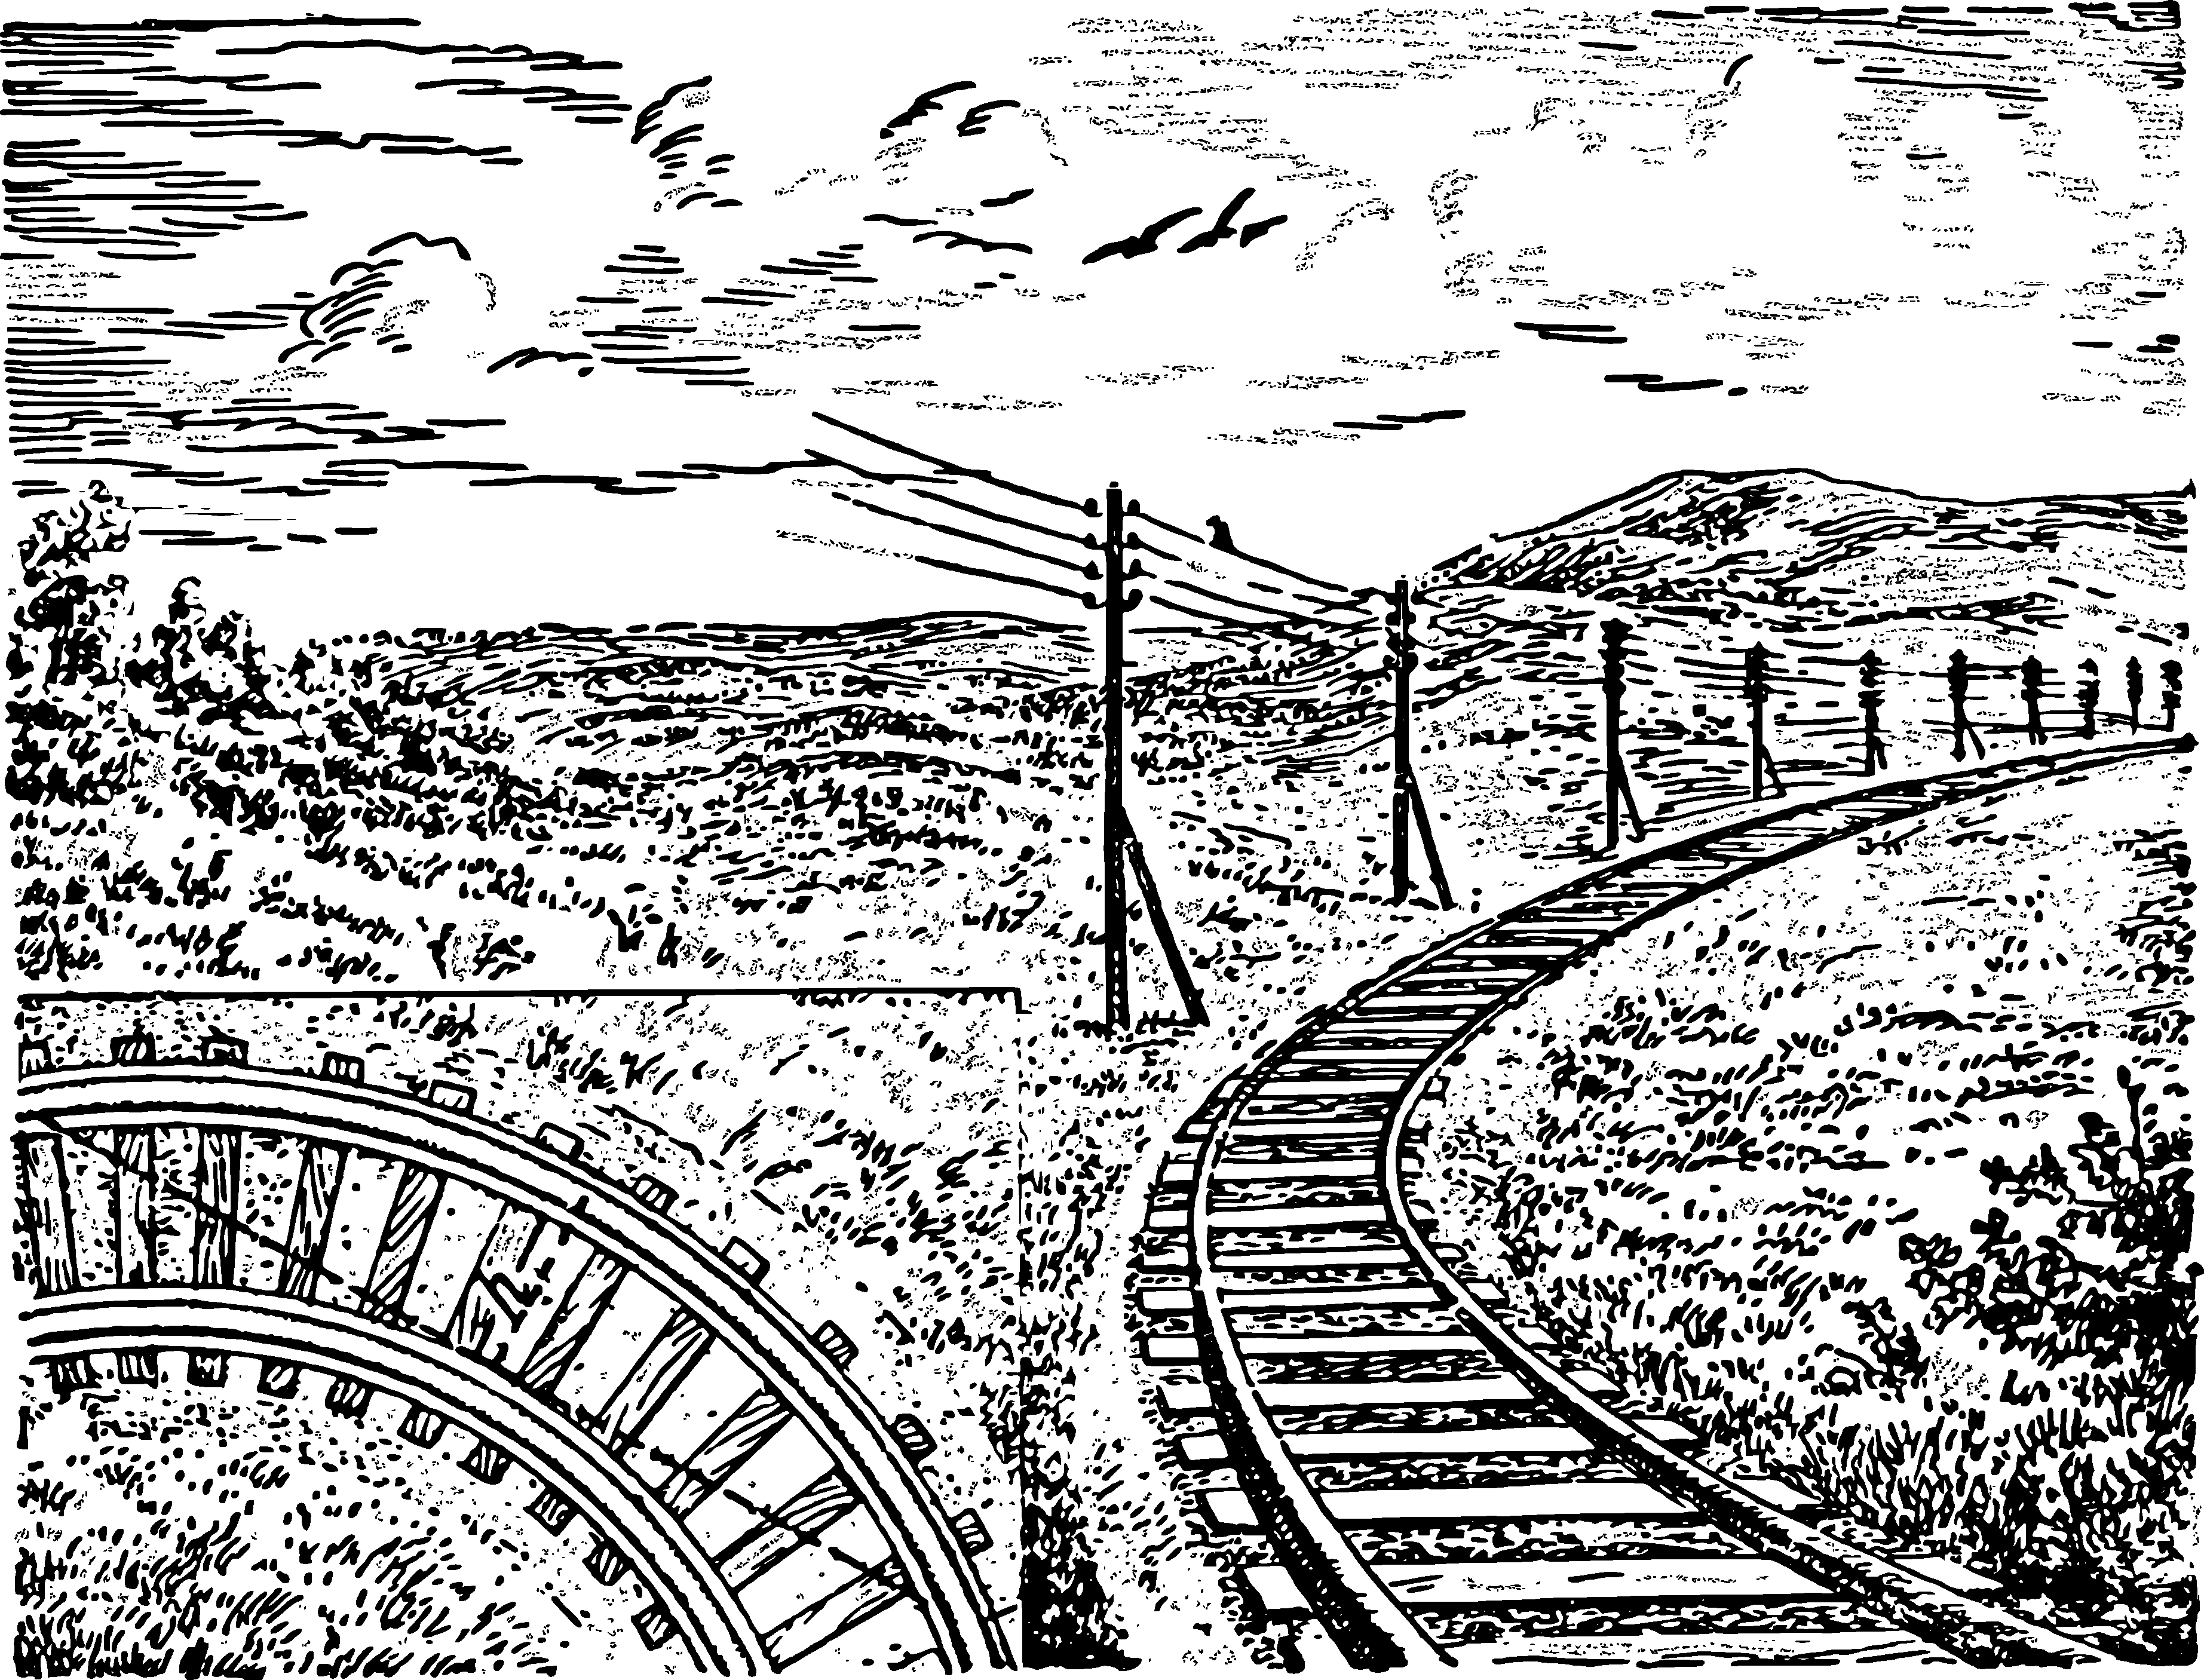
\includegraphics[width=\textwidth]{figures/ch-04/fig-085.pdf}
\sidecaption{Calculating the radius of a railway curve.\label{fig-085}}
\end{figure}

If rails are laid on the road, then finding the radius of curvature is simplified. In fact, by stretching a rope along the tangent to the inner rail, we get the chord of the arc of the outer rail, the arrow of which h (\figr{fig-085}) is equal to the gauge of the track -- \SI{1.52}{\meter}. The radius of curvature in this case (if a is the length of the chord) is approximately
\begin{equation*}%
R = \frac{a^{2}}{8 \times 1.52} = \frac{a^{2}}{12.2}
\end{equation*}
For $a = \SI{120}{\meter}$, the radius of curvature is \SI{1200}{\meter}.\sidenote{In practise, this method presents the disadvantage that, due to the large radius of rounding, the rope for the chord requires a very long one.}




\section{The bottom of the ocean}
\label{sec-4.8}

The analogy of a road curve to the bottom of the ocean seems like a somewhat unexpected leap, at least not immediately clear. However, geometry ties both topics together quite naturally.

\begin{marginfigure}%[-3cm]%[h!]
\centering
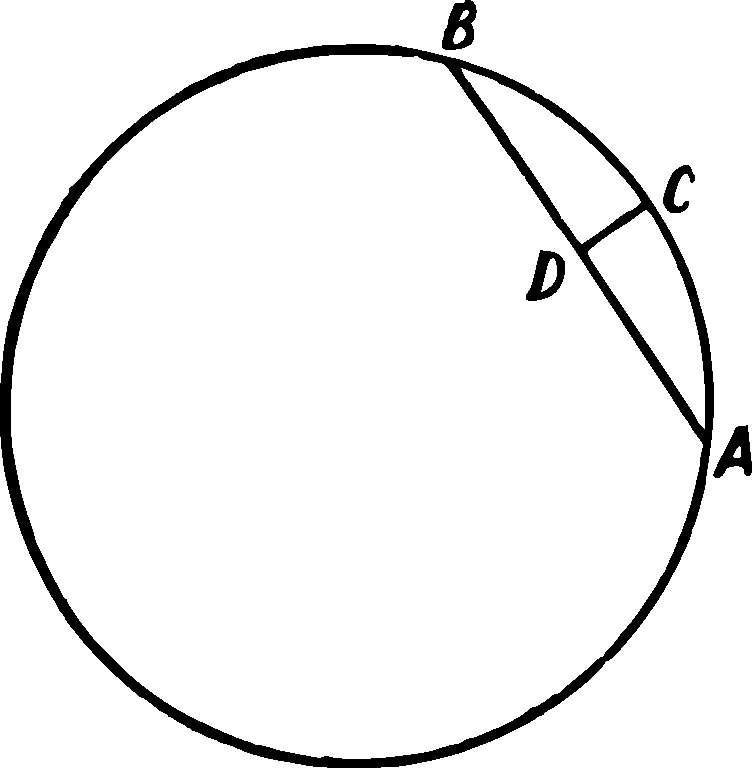
\includegraphics[width=\textwidth]{figures/ch-04/fig-086.pdf}
\sidecaption{Is the ocean floor flat.\label{fig-086}}
\end{marginfigure}

We are talking about the curvature of the ocean floor, what shape it takes: concave, flat, or convex. To many, it will undoubtedly seem incredible that despite their immense depth, the oceans do not form basins on the Earth's surface; as we will see, their bottom is not only not concave but even convex. Considering the ocean as ``bottomless and boundless'', we forget that its ``boundlessness'' is hundreds of times greater than its ``bottomlessness'', i.e., the water depth of the ocean represents a far-reaching layer that, of course, mirrors the curvature of our planet.

Let's take the example of the Atlantic Ocean. Its width near the equator is approximately one-sixth of the full circumference. If the circle in \figr{fig-086} is the equator, then arc $ACB$ represents the water expanse of the Atlantic Ocean. If its bottom were flat, the depth would equal $CD$, the arrow of arc $ACB$. Knowing that arc $AB = 1/6$ of the circumference and, consequently, chord $AB$ is a side of a regular inscribed hexagon (which, as is known, equals the radius of the circle $R$), we can calculate $CD$ from the previously derived formula for road curves:
\begin{equation*}%
R = \frac{a^{2}}{8h}, \qor h = \frac{a^{2}}{8R}
\end{equation*}
Knowing that $a = R$, we get for this case we get $h = R/8$. With $R = \SI{6400}{\kilo\meter}$, we have: $h = \SI{800}{\kilo\meter}$.

Thus, for the bottom of the Atlantic Ocean to be flat, its greatest depth should be 800 km. In reality, however, it does not even reach 10 km. Hence the straightforward conclusion: the bottom of this ocean, in its general form, exhibits convexity, slightly less curved than its water surface.

This holds true for other oceans as well: their bottoms represent areas of reduced curvature on the Earth's surface, hardly deviating from its overall spherical shape.

Our formula for calculating the radius of road curvature shows that the larger the water basin, the more convex its bottom. Looking at formula $h = a^{2}/8R$, we directly see that with increasing width $a$ of the ocean or sea, its depth $h$ must increase very rapidly, proportional to the square of width $a$. However, when transitioning from smaller water basins to larger ones, depth does not increase in such a swift progression. 

An ocean may be a hundred times wider than a sea, but its depth is not a $100 \times 100$, i.e., ten thousand times deeper. Therefore, relatively smaller basins have bottoms more depressed than oceans. The bottom of the Black Sea between Crimea and Asia Minor is not convex like oceans, not even flat but slightly concave. The water surface of this sea represents an arc approximately \ang{2} (more precisely, 1/170 of the Earth's circumference). The depth of the Black Sea is quite uniform and equals \SI{2.2}{\kilo\meter}. Equating the arc to the chord in this case, we find that for it to have a flat bottom, the sea should have a maximum depth of approximately 
\begin{equation*}%
h = \frac{40000^{2}}{ 170^{2} \times 8R} = \SI{1.1}{\kilo\meter}.
\end{equation*}
Thus, the actual bottom of the Black Sea lies more than one kilometre $(2.2 - 1.1)$ below the imagined plane drawn through the extreme points of its opposite shores, i.e., it represents a basin, not convexity.

\clearpage

\section{Do water mountains exist?}
\label{sec-4.9}


The previously derived formula for calculating the radius of road curvature will help us answer this question.

The previous problem has already prepared us for the answer. Water mountains exist, but not in the physical sense of these words, but rather in their geometric meaning. Not only each sea but even each lake represents, in a way, a water mountain. 

\begin{figure}[h!]
\centering
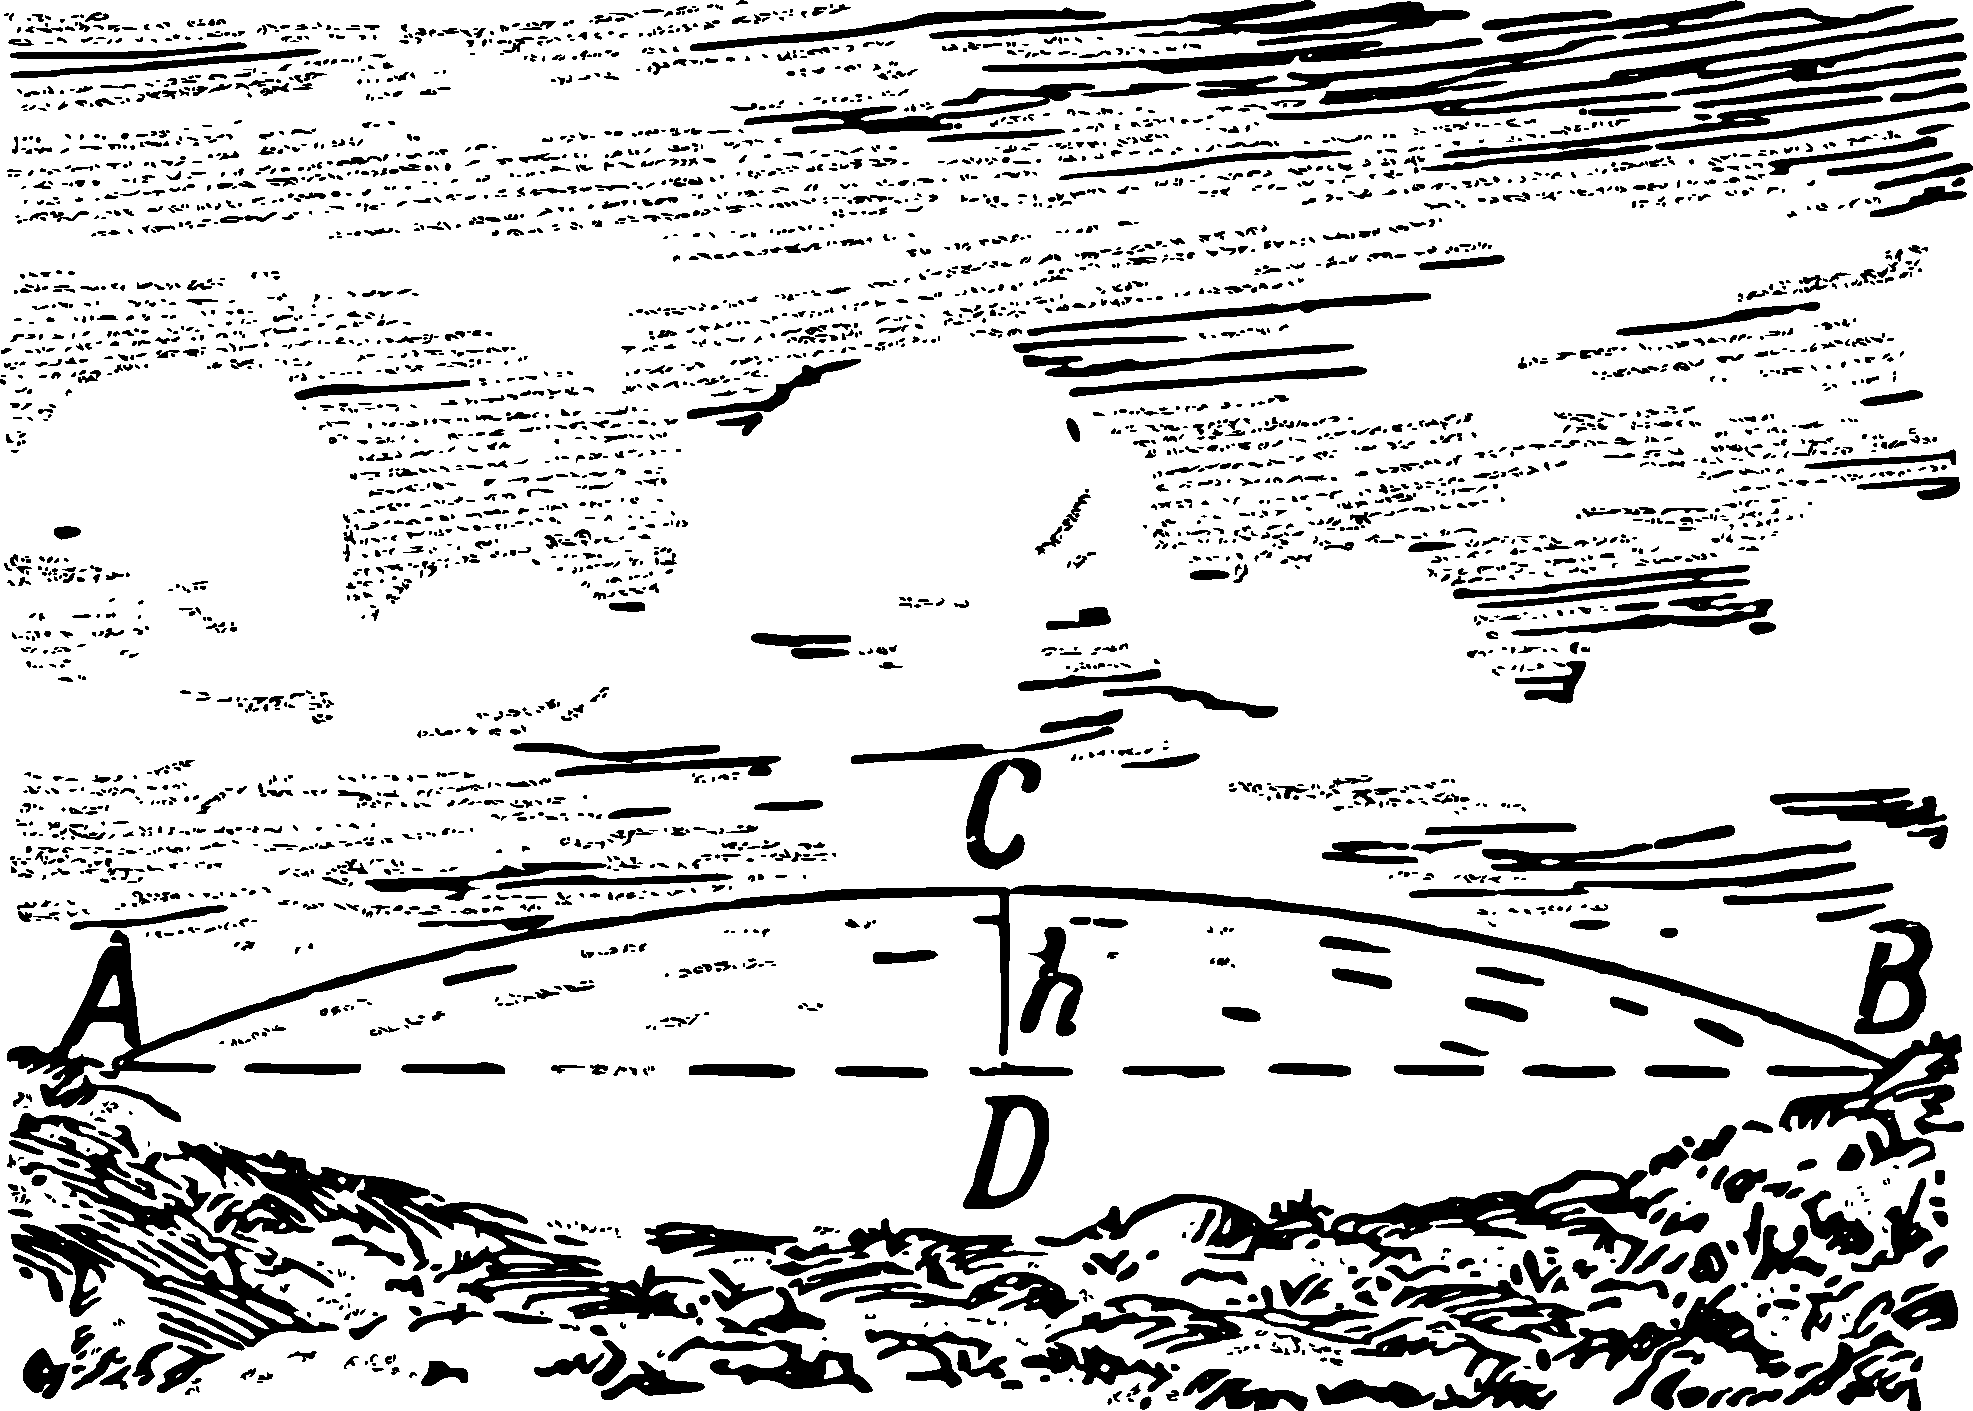
\includegraphics[width=0.8\textwidth]{figures/ch-04/fig-087.pdf}
\sidecaption{``The Water Mountain.''\label{fig-087}}
\end{figure}

When you stand at the shore of a lake, you are separated from the opposite shore by a convexity of water, the height of which is greater the wider the lake. We can calculate this height: using the formula $R = a^{2}/8h$, we have the value of the depth $h = a^{2}/8R$. Here, $a$ is the distance between the shores in a straight line, which we can equate to the width of the lake (chord-arc). If this width, let's say, is 100 km, then the height of the water ``mountain'' is about 200 meters.
\begin{equation*}%
h = \frac{10000}{8 \times 6400} = \SI{200}{\meter}.
\end{equation*}
A water mountain of impressive height!

Even a small lake with a width of 10 km elevates the peak of its convexity above the straight line connecting its shores by 2 meters, i.e., higher than human height.




But are we right to call these water convexities ``mountains''? In the physical sense, no: they do not rise above the horizontal surface, so they are plains. It is erroneous to think that the line $AB$ (\figr{fig-087}) is a horizontal line over which arc $ACB$ rises. The horizontal line here is not $AB$, but $ACB$, coinciding with the free surface of calm water. The line $ADB$ is inclined to the horizon: $AD$ slopes downward underground to point $D$, its deepest point, and then rises up again, emerging from the ground (or water) at point $B$. If pipes were laid along the line $AB$, a ball placed at point $A$ would not stay here, but would roll (when the pipe walls are smooth) to point $D$ and from there, picking up speed, would ascend to point $B$; then, unable to stay there, it would roll back to $D$, run to $A$ again, roll down again, and so on. An ideally smooth ball in an ideally smooth pipe (with no air hindering movement) would roll back and forth endlessly\dots{}

So, although it may seem to the eye (\figr{fig-087}) that $ACB$ is a mountain, in the physical sense of the word, it is a flat area. The mountain -- if you will -- exists here only in a geometric sense.


\begin{center}
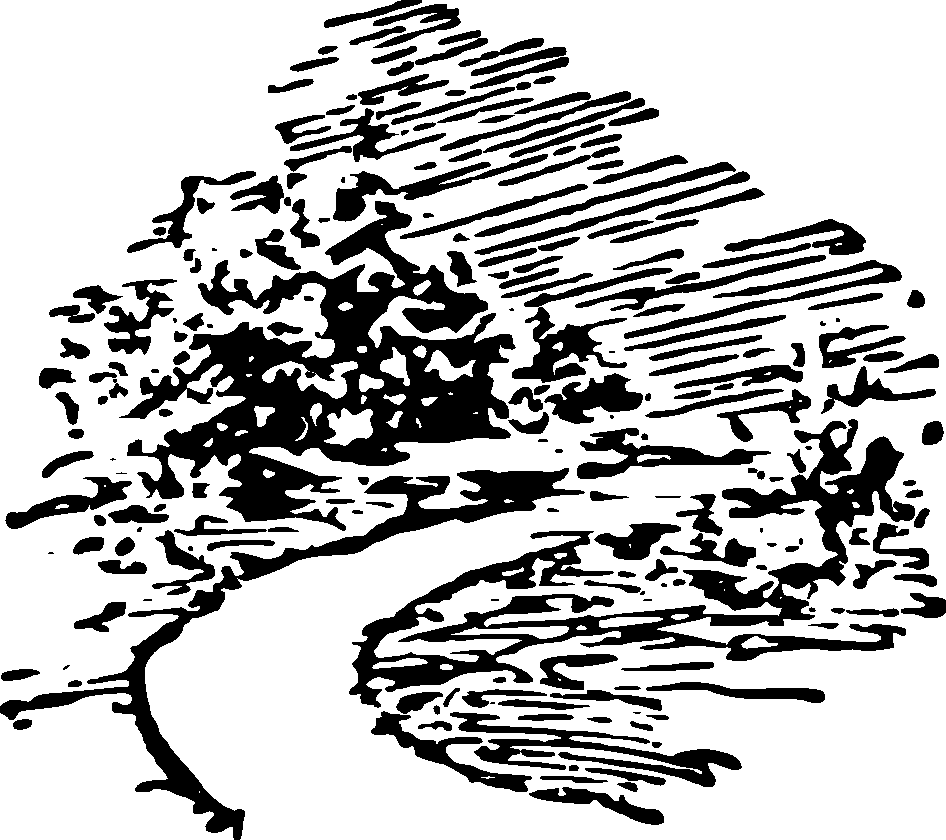
\includegraphics[width=0.3\textwidth]{figures/ch-04/fig-ch-04-tail.pdf}
\end{center}


















